\documentclass[twocolumn,spanish]{revtex4-1}
\usepackage[spanish]{babel}
\usepackage[utf8]{inputenc}
\usepackage{amsmath,amssymb}
\usepackage{lipsum}
\usepackage{float}
\usepackage{subcaption}
\usepackage{hyperref}
\usepackage{cleveref}

\usepackage{algorithm}
\usepackage{algpseudocode}
\makeatletter
\renewcommand{\ALG@name}{Algoritmo}
\makeatother
\algrenewcommand\algorithmicfor{\textbf{para}}
\algrenewcommand\algorithmicwhile{\textbf{mientras}}
\algrenewcommand\algorithmicdo{\textbf{hacer}}
\algrenewcommand\algorithmicend{\textbf{fin}}
\algrenewcommand\algorithmicif{\textbf{si}}
\algrenewcommand\algorithmicthen{\textbf{entonces}}

\usepackage{graphicx}
\graphicspath{{images/}}

\usepackage{fancyhdr}
\pagestyle{fancy}

\usepackage{tikz}
\usetikzlibrary{babel, arrows.meta, matrix}
\decimalpoint


\renewcommand{\figurename}{{\bf Fig.}}
\renewcommand{\tablename}{{\bf Tabla}}
% \renewcommand{\thesection}{\arabic{section}}
% \renewcommand{\thesubsection}{\arabic{subsection}}


\begin{document}
\title{Neuroevolución concurrente para el juego de Flappy Bird}
\author{Barrero, P.}
\author{Figueroa, R.}
\author{Hernández, A.}
\author{Padilla, A.}
\date{10 de Febrero del 2021}
\affiliation{Computación Concurrente - IIMAS\\Universidad Nacional Autónoma de México}

\begin{figure}
    \flushleft 
\includegraphics[width=1in]{unam_logo.jpg}
\end{figure}
\begin{figure}
    \flushright 
\includegraphics[width=1in]{logoiimas.png}
\end{figure}
\begin{abstract}   %%Resumen
\begin{center}
\textbf{Abstract} \\
\end{center}

En este trabajo se presentan los conceptos básicos de los algoritmos bio-inspirados y evolutivos, de los cuales se explican los algoritmos de colonia de hormigas, de banco de peces y de neurevolución así como algunas de sus aplicaciones. Posteriormente se escoge el algoritmo de neuroevolución para aplicarlo al juego de Flappy Bird. Con la aplicación del algoritmo de neuroevolución se realiza su implementación de manera paralela para mejorar su rendimiento y se evalúa la mejora en speed-up comparando la implementación concurrente y la secuencial.

\end{abstract}

\maketitle


%%%%%%%%%%%%%%%%%%%
%\onecolumngrid

%%%%%%%%%%%%%%%%%%%
\section{Introducción}

No son pocas las dificultades que se presentan en problemas de optimización de gran escala, los gradientes por descenso pueden estancarse en mínimos locales, los espacios de búsqueda pueden ser demasiado grandes para explorarlos exhaustivamente entre muchas otras posibles complicaciones. Por estas razones es que se han desarrollado soluciones que utilizan algoritmos inspirados en los seres vivos y su comportamiento, estos algoritmos imitan algunas de las características de los seres vivos como pueden ser el aprendizaje, la adaptación y la evolución \cite{krishnanand2009comparative}.

En general los Algoritmos Evolutivos y Bioinspirados (AEB) pueden tratar de replicar tanto el comportamiento, individual y en colectividad de lo seres vivos, como cualidades físicas y genéticas como puede ser la evolución o las producción de feromonas.

Entre los algoritmos bioinspirados destaca como los científicos de la computación han utilizado el comportamiento de las colonias de abejas, las parvadas de pájaros, los bancos de peces, entre otras colectividades animales para resolver otros tipos de problemas. Este tipo de fenómenos exhiben características como la escalabilidad, la autonomía, la adaptación, el paralelismo y la tolerancia a las fallas que son de gran valor en las soluciones que se proponen con este tipo de algoritmos. Este tipo de algoritmos ha dado origen a la llamada inteligencia de colmena que es un subcampo de la inteligencia artificial \cite{darwish2018bio}.

Los algoritmos genéticos son una herramienta que puede aplicarse al aprendizaje automático para encontrar buenas soluciones a problemas que tienen una gran cantidad de posibles soluciones. Esta metaheurística bioinspirada, toma conceptos de los procesos biológicos al generar candidatos a soluciones, los cuales evalúa respecto al resultado deseado y va refinando las mejores soluciones \cite{sheppard}.

La idea fundamental es los algoritmos evolutivos es mantener un conjunto de candidatos que representen una posible solución al problema. Estos se mezclan y compiten entre sí, siguiendo el principio de selección natural. Por tanto los individuos más `aptos’ tienen mayor longevidad y por ende mayor probabilidad de generar nuevos candidatos, simulando la reproducción \cite{Andaluz}.

El rendimiento de las estrategia evolutivas depende de la selección de parámetros así como la evolución de los mismos. Los operadores más importantes para este conjunto de técnicas son la selección, mutación, recombinación y elitismo, siendo el segundo de los mencionados el operador primario en un algoritmo evolutivo, a diferencia de los algoritmos genéticos. Cabe señalar que algunos parámetros pueden estar fijos durante la evolución del algoritmo, a estos se les nombra parámetros exógenos, y por otro lado están los parámetros endógenos que están codificados dentro del mismo individuo \cite{Matlab}. 


\section{Algoritmos Evolutivos y Bioinspirados}

\subsection{Colonia de hormigas}

Los algoritmos de colonias de hormigas o ACO, \textit{Ant Colony Optimization}, están basados en la forma en que las hormigas se organizan para recolectar comida, las cuales dejan caminos de feromonas detrás suyo. Cuando las trabajadoras encuentran comida, estas regresan al nido, reforzando el camino marcado. En caso de que haya dos caminos hacia la comida, las hormigas seleccionaran de manera aleatoria la ruta, sin embargo, al pasar el tiempo, el camino más corto será reforzado, figura \ref{fig:hormigasyumyum}. Asimismo, otras hormigas se verán más atraídas por las trayectorias que tengan rastros más fuertes de feromonas, mediante este método, la colonia encontrará rápidamente recursos y una gran cantidad de sus trabajadoras llegarán a estos por los caminos más eficientes  \cite{fan2020review}.

\begin{figure}[h]
    \centering
    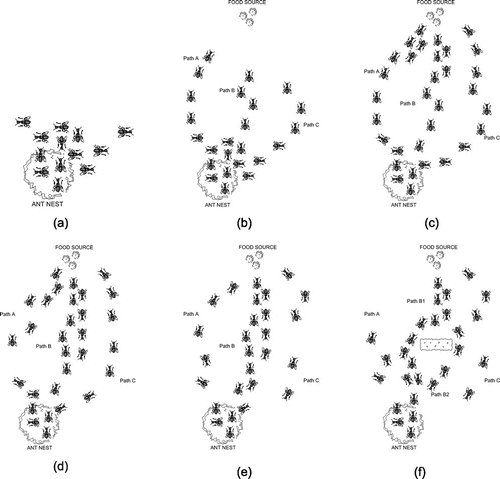
\includegraphics[width=0.45\textwidth]{hormigas}
    \caption{Comportamiento de una colonia de hormigas buscando comida. a) Nido de hormigas b) Las hormigas empiezan a dirigirse a la fuente de alimentos por varios caminos c) Las hormigas llegan a la comida, dejando su rastro de feromonas en el camino d) En el camino más corto existió una mayor concentración de feromonas por lo que algunas hormigas empiezan a preferir ese camino e) Gran parte de las hormigas se van por el camino óptimo f) Las trabajadoras se adaptan a los obstáculos \cite{christodoulou2010scheduling}.}
    \label{fig:hormigasyumyum}
\end{figure}
% Holi
\subsubsection{Funcionamiento}

La idea general del algoritmo consiste de varias hormigas artificiales que trazarán un camino en un espacio de soluciones en cada iteración, este espacio está compuesto por nodos que representan las soluciones y aristas entre los nodos, dirigidos hacia el objetivo. Las hormigas no pueden visitar de nuevo un nodo, y en cada paso el camino se selecciona a través de un mecanismo estocástico que se encuentra sesgado por una variable que representa a la feromona, la cual ésta asociada a cada arista y que las hormigas pueden leer \cite{dorigo2019ant}.

En la figura \ref{fig:ACOAlgorithm} se muestra un esquema general de la metaheurística de la colonia de hormigas como aplicación para problemas estocásticos de combinatoria. Después de inicializar los parámetros y los caminos de feromonas, el ciclo principal se mantiene en los tres pasos esenciales. Primero $m$ hormigas construyen soluciones a la instancia del problema que estemos considerando. Una vez completadas las soluciones, estas deberían mejorarse y finalmente, antes de iniciar la siguiente iteración, los caminos de feromonas se modifican con tal de que reflejen las experiencias de búsqueda de las hormigas \cite{dorigo2019ant}. 

\begin{figure}
    \centering
    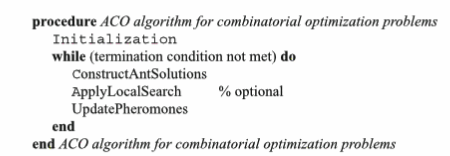
\includegraphics[width=0.9\linewidth]{ACOalgorithm}
    \caption{Estructura general del algoritmo ACO \cite{dorigo2019ant}}
    \label{fig:ACOAlgorithm}
\end{figure}

\subsubsection{Casos de uso}

Dada su naturaleza, las estrategias y algoritmos inspirados han encontrado mucha aplicaciones en problemas de combinatoria discreta \cite{6281180}.

\begin{itemize}
    \item \textbf{El problema del agente viajero.}\\
    EL problema del agente viajero, TSP por sus siglas en inglés, es uno que ha generado mayor cantidad de investigación al tratarse de un problema NP-duro. El TSP también ha jugado un rol importante en el desarrollo de la investigación en ACO, pues el primer algoritmo de colonia de hormigas, llamado \textit{Ant SYstem} fue empleado primero en el problema del agente viajero \cite{dorigo1996ant,dorigo2019ant}. En ese primer trabajo, aparte de resultar un algoritmo 'intuitivo' que se adaptaba naturalmente al problema, demostró resultados positivos, sin embargo, resultaron ser inferiores a los algoritmos en un estado del arte de la época. Sin embargo esto dio pauta al desarrollo de algoritmos ACO, con algunos encontrando aplicaciones de la vida real como vigilancia de la vida silvestre \cite{chowdhury2019modified}.
    
    \item \textbf{Problema de enrutamiento de vehículos.}\\
    EL problema de enrutamiento de vehículos es uno que está relacionado con el problema del agente viajero. Este consiste en que dado un conjunto de vehículos y un conjunto de locaciones, se busca un camino que recorra todas las locaciones con un costo mínimo \cite{bonilha2020ant}.
    
    \item \textbf{Detección de bordes en imágenes.}\\
    Hay artículos donde se ha propuesto el uso de algoritmos de búsqueda de colonia de hormigas, siendo que la imagen se modelo como una gráfica donde cada nodo representaba un pixel. Los experimentos realizados sugirieron la efectividad del uso de esta estrategia \cite{nezamabadi2006edge}.
\end{itemize}

\subsection{Algoritmo de Banco de Peces}
El  algoritmo de banco de peces toma su inspiración del comportamiento de los pescados, donde cada pescado busca comida por su cuenta de manera individual mientras que cada pez puede comunicarse con otros peces para llegar a una optimización global en la obtención de alimentos. De esta manera se puede construir un algoritmo que explore un espacio de soluciones $D$ dimensional, con $N$ peces. Cada uno de estos pesos tiene una ubicación en el espacio $X=(x_1,x_2,x_3,\cdots,x_D)$, de tal forma que se puede definir una función de aptitud $Y_i=f(X_i)$ que nos representa que tan buen acceso a alimento tiene algún pez dado. Cada pez tiene cierto rango visual y puede comportarse en fases de caza, banco y de seguimiento \cite{darwish2018bio,neshat2012review}.

\subsubsection{Funcionamiento}
El algoritmo comienza colocando a los $N$ peces en posiciones aleatorias y estos empiezan en la fase de caza. En la fase de caza cada pez selecciona una posición aleatoria $X_{j}$ en su rango visual y si esta posición aleatoria contiene más alimento $Y_j > Y_i$, entonces el pez se mueve un paso en esta dirección. Esta fase puede describirse como:

\begin{equation*}
    X_i^{t+1} = 
    \begin{cases}
     X_i^{t} + \textbf{paso}\times \frac{X_j-X_i^t}{||X_j-X_i^t||} & Y_j > Y_i\\
     \text{movimiento aleatorio} & \text{en otro caso}
    \end{cases}
\end{equation*}

Donde $X_i^{t+1}$ es la posición al siguiente paso y $X_i^{t}$ es la posición actual de algún pez dado.

Posteriormente los peces entran en fase de banco, donde evalúan si el punto central $c$ de los peces que están en su alcance visual tiene una mayor concentración de comida que la que tiene él, para esto verifica si $Y_c/N_{\text{vecinos}} > \delta Y_i$, donde $\delta$ es un factor de multitud. De tal forma que este comportamiento se puede definir como:

\begin{equation*}
    X_i^{t+1} = 
    \begin{cases}
     X_i^{t} + \textbf{paso}\times \frac{X_c-X_i^t}{||X_c-X_i^t||} & \ \frac{Y_c}{N_{\text{vecinos}}} > \delta Y_i\\
     \text{fase de caza} & \text{en otro caso}
    \end{cases}
\end{equation*}

Finalmente los peces también pueden comportarse en fase de seguimiento, en la cual se dirigen hacia la posición con mejor cantidad de alimento si puede conseguir si el alimento por pez tiene un mejor rendimiento que el dado por su factor de multitud, es decir, si   $Y_{\text{mejor}}/N_{\text{vecinos}} > \delta Y_i$. Con esto en mente esta fase puede describirse como:

\begin{equation*}
    X_i^{t+1} = 
    \begin{cases}
     X_i^{t} + \textbf{paso}\times \frac{X_{\text{mejor}}-X_i^t}{||X_c-X_i^t||} & \frac{Y_{\text{mejor}}}{N_{\text{vecinos}}} > \delta Y_i\\
     \text{fase de caza} & \text{en otro caso}
    \end{cases}
\end{equation*}

Con este algoritmo inspirado en bancos de peces, sus comportamientos individuales y grupales, se puede explorar eficazmente el espacio de soluciones de un problema complejo.

\subsubsection{Casos de uso}

Algunas aplicaciones del algoritmo de banco de peso pueden ser \cite{neshat2012review}:

\begin{itemize}
    \item \textbf{Planificar trabajo de múltiples robots:} El algoritmo de banco de peces ha sido usado para minimizar la desviación entre el uso de recursos y los niveles objetivo de un grupo de varios robots autónomos. Los resultados de este estudio mostraron buenos resultados, convergencia rápida a la solución, insensibilidad a las condiciones iniciales y una implementación sencilla \cite{tian2009improved}.
    
    \item\textbf{Optimizar los parámetros de controladores PID:} Los controladores PID son ampliamente usados en la industria y aplicaciones tecnológicas, sin embargo, encontrar los parámetros óptimos para este tipo de controladores no es tarea fácil, por lo que entre las heurísticas que se han utilizado para encontrarlas el utilizar el algoritmo de banco de peces \cite{luo2010optimization}.%HOLI
\end{itemize}

\subsection{Algoritmo de Neuroevolución.}

Los algoritmos de neuroevolución forman parte de la familia de los algoritmos genéticos (AG). En este tipo de AG busca minimizar la función de costo de una red neuronal por métodos alternativos al descenso por gradiente. Para hacer esto se utiliza aprendizaje por refuerzo.  Una ventaja de este tipo de algoritmos es que solo requieren de una métrica de rendimiento para cada uno de los miembros de la población que se está simulando \cite{such2017deep}. 

\subsubsection{Funcionamiento}
Un algoritmo genético evoluciona una población $P$ de $N$ individuos. Estos individuos en el caso de la neuroevolución están caracterizados por los pesos de su red neuronal $\theta$, en el contexto de los algoritmos genéticos $\theta$ es el genotipo (cromosomas) de cada individuo. El conjunto de cromosomas de cada individuo evoluciona, por lo que $\theta_i$ indica los pesos de la generación $i$, para cada generación podemos obtener una función de aptitud (fitness) $F(\theta_i)$ la cual indica que tan buen rendimiento tiene un individuo de la generación $i$ para una tarea dada. 

Existen varias técnicas de realizar la evolución cromosómica entre generaciones \cite{such2017deep,Montana1989TrainingFN}, entre ellas se encuentra la evolución entre generaciones que consiste en hacer que los $T$ individuos con mayor aptitud de una generación dada sean los que den origen (sean padres) a los individuos de la generación siguiente. Para generar un hijo se toma a un padre de los $T$ individuos seleccionados en la generación de manera aleatoria y se les aplica a sus cromosomas una función de deriva genética que consiste en agregar ruido gaussiano a sus cromosomas o un subconjunto de estos, de tal forma que los cromosomas del hijo se vuelve $\theta_{i+1}=\theta_i + \sigma \epsilon$, donde $\sigma$ es un parámetro que se puede determinar de manera empírica mientras que $\epsilon = N(0, I)$ tiene distribución normal, con $I$ la desviación estándar de cada mutación. Otra manera de crear mutaciones es remplazando un subconjunto de los cromosomas con nuevos valores aleatorios. Este proceso se repite para una cantidad deseada $N-u$ de individuos. La siguiente generación puede tener $u$ individuos que tengan exactamente los mismos cromosomas de los mejores individuos de la generación anterior en un proceso llamado elitismo.

Para realizar la cruza entre individuos también existen varias opciones entre las que se encuentra la cruza ingenua lineal, la cual consiste que en lugar de tomar un único padre, podemos tomar dos ($a$ y $b$) y generar los cromosomas de sus hijos como $\theta_{i+1}=(1-t)\theta_a + t \theta_b$  con t un parámetro que determina que tanto se influirá en la cruza cada padre. Este tipo de cruza se considera no segura y suele llevar a descendencia dañada \cite{uriot2020safe}, sin embargo, podría ser útil en redes pequeñas. Otra opción de cruza es simplemente hacer una elección aleatoria de los pesos de los padres de tal forma que los hijos contienen una fracción de los cromosomas de cada padre \cite{Montana1989TrainingFN}, en este tipo de cruza existen diferentes variantes dependiendo como se eligen los cromosomas de cada padre.

En cuanto a los métodos de selección destacan el método del torneo, en el cual se escogen aleatoriamente $k$ individuos del total de individuos de la población, los cuales serán los concursantes del torneo. Con base a la función de aptitud de cada individuo escogido se seleccionan $m$ individuos con mejor aptitud los cuales son los que ganan el torneo \cite{blickle1996comparison}. Otra manera de realizar selección es el método de la ruleta o el método proporcional, en el cual se escogen aleatoriamente $k$ individuos, la suma total de la función de aptitud de estos es $sum_{apt}$, de tal forma que se les asigna una probabilidad $w_i=\frac{apt_i}{sum_{apt}}$ al $i$ésimo individuo escogido. Con estas probabilidades se construye un segmento de linea con longitudes consecutivas igual a las $w_i$, de tal forma que se elige posteriormente un número aleatorio entre 0 y 1 y dependiendo de donde caiga este número aleatorio es el individuo que se selecciona para reproducirse \cite{lipowski2012roulette}. La selección por ruleta se ilustra en la figura \ref{fig:roulette}.

\begin{figure}[ht]
\centering
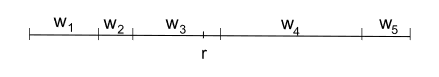
\includegraphics[width=8cm]{ruleta.png}
\begin{quote}
\caption{Segmento de linea construido con las probabilidades de selección de cada individuo escogido y el valor $r$ generado aleatoriamente para determinar cual de ellos seleccionar \protect\cite{lipowski2012roulette}}
\label{fig:roulette}
\end{quote}
\end{figure}

\subsubsection{Casos de uso}
Algunas aplicaciones notables del algoritmo de neuroevolución son:

\begin{itemize}
    \item \textbf{Simular la dinámica de la caminata bipeda:} Con el algoritmo de neuroevolución se ha logrado entrenar redes neuronales para que puedan controlar a un modelo humanoide de tal manera que este camine de manera veloz sin que pierda el equilibrio \cite{jackson2019neuroevolution}. Este tipo de aplicación se ilustra en la figura \ref{fig:bipedo}.
    \item \textbf{Conducción autónoma:} Con neuroevolución también se han logrado entrenar redes neuronales para manejar de manera autónoma vehículos automotores \cite{sainathapplication}. La conducción autónoma es una rama de la investigación científica que ha aumentado de popularidad y una aplicación ingenieril cada vez más tangible e inminente.
\end{itemize}

\begin{figure}[h]
    \centering
    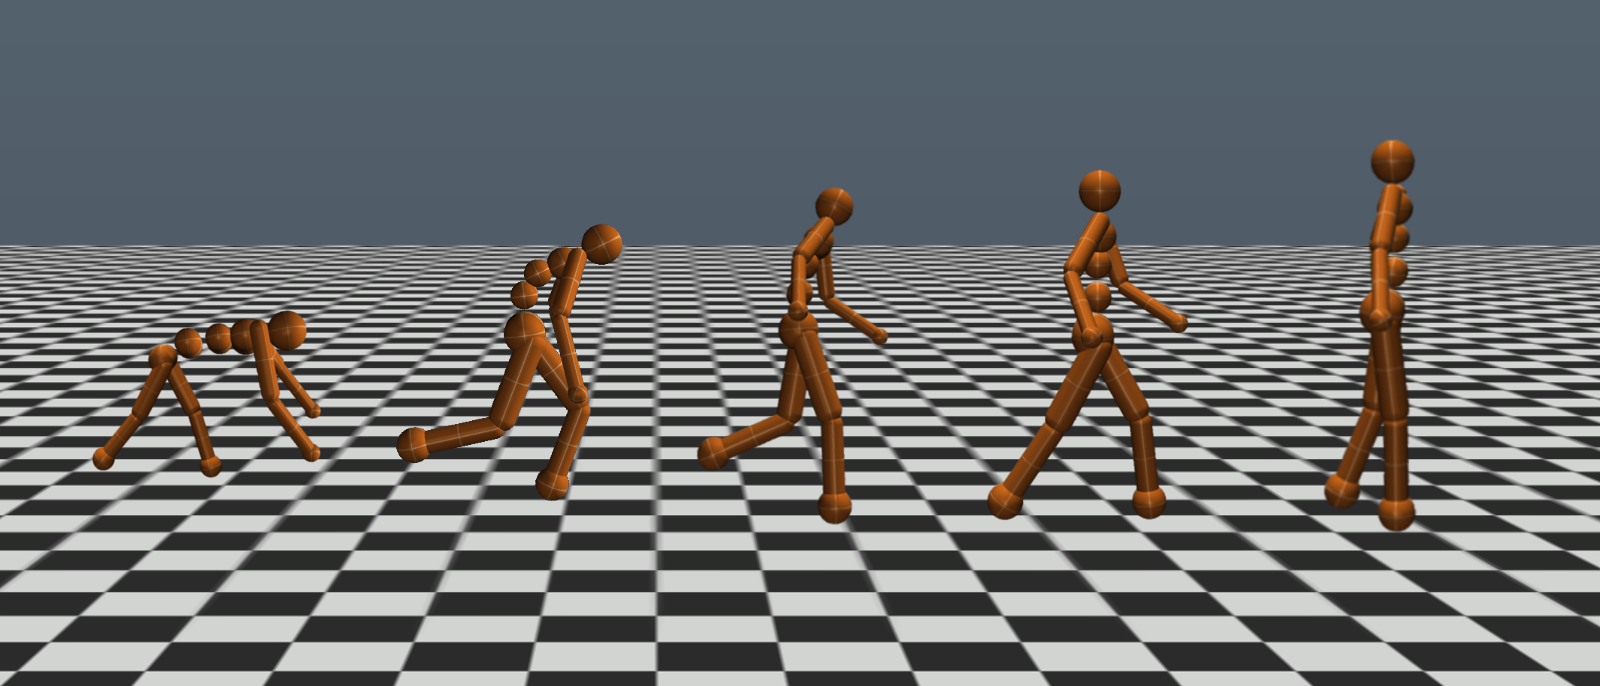
\includegraphics[width=0.9\linewidth]{images/neuroevol.png}
    \caption{El algoritmo de neuroevolución ha sido usado para enseñarle modelos humanoides a caminar \protect\cite{stanley2017welcoming}}
    \label{fig:bipedo}
\end{figure}

\subsection{Redes Neuronales}
Una red neuronal artificial son un modelo computacional que ha ido evolucionando a través de la historia, y que en los últimos años ha obtenido mucha popularidad debido a la cantidad de problemas que pueden resolver.

Una red neuronal artificial consta de una serie de capaz, cada capa consta de una serie de neuronas y una función de activación. Cada neurona posee un real. La idea de una red es convertir una serie de entradas en una salida. 

\subsubsection{Operaciones genéticas sobre redes neuronales}\label{sec:codificacion}

\textbf{Codificación y decodificación}

La codificación es una forma en representar redes neuronales complejas como un vector unidimensional, para facilitar operaciones como el intercambio o actualización de pesos. 

\begin{figure}[ht]
    \centering
    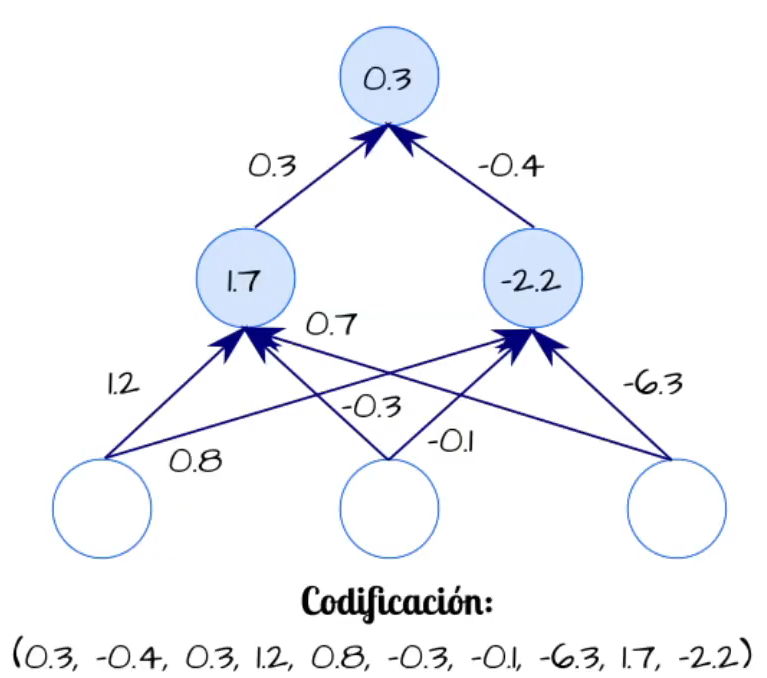
\includegraphics[width=0.9\linewidth]{images/codificacion.png}
    \begin{quote}
    \caption{Ejemplo de codificación de una red neuronal 
    \protect\cite{profa}}
    \end{quote}
    \label{fig:condificacion}
\end{figure}

Si las capas de una red neuronal están representadas como un conjunto de pesos en la forma de una matriz bidimensional, y un conjunto de \textit{bias} como un vector de una dimensión, una algoritmo de codificación fácil de implementar es el siguiente:
\begin{enumerate}
    \item Volvemos todas las matrices de pesos vectores unidimensionales (por ejemplo, concatenando fila por fila, o columna por columna).
    \item Concatenamos cada vector de peso con su correspondiente vector de \textit{bias}.
    \item Concatenamos todos los vectores resultantes, empezando por la entrada de la red neuronal.
\end{enumerate}

La operación inversa a la codificación se conoce como \textbf{decodificación}. Naturalmente, para poder decodificar un cromosoma, se necesitan saber las propiedades del individuo (en el caso del ejemplo anterior el tamaño de cada una de las capas).

\textbf{Mutación}

En esta operación se tiene como entrada un cromosoma y una salida que es un cromosoma también. Para cada entrada de un cromosoma se le suma un pequeño ruido con probabilidad $p$. En el siguiente ejemplo aplicamos una mutación con $p=0.1$.

\begin{figure}[H]
    \centering
    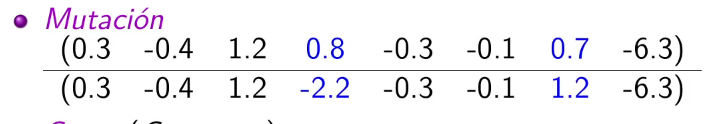
\includegraphics[width=0.9\linewidth]{images/mutacion.png}
    \begin{quote}
    \caption{Ejemplo de una mutación en una red neuronal 
    \protect\cite{profa}}
    \end{quote}
    \label{fig:mutacion}
\end{figure}

\textbf{Cruza}

En esta operación se tienen dos cromosomas $A, B$ del mismo tamaño como entrada a los que les denota como padres y como salida uno o varios cromosomas $C$. Existen varias cruzas, como por ejemplo:

\begin{enumerate}
    \item Cruza común\\
        En esta operación tenemos dos cromosomas $A, B$ como entrada y un cromosoma de salida $C$, $C[i]$ valdrá lo siguiente:\\
        \begin{equation*}
            C[i]=
            \begin{cases}
                A[i] &  \text{si}\ U[i]<p \\
                B[i] & \text{en otro caso} \\
            \end{cases}
        \end{equation*}
        donde $p$ es la probabilidad de elegir una característica (peso/sesgo) del padre $A$, y $U[i]$ es una variable aleatoria uniforme entre $0$ y $1$. Cuando $p=0.5$ se le conoce como \textbf{Cruza Uniforme}.
        
        En la figura $7$ se puede ver un ejemplo de la cruza común.
        \begin{figure}[H]
        \centering
        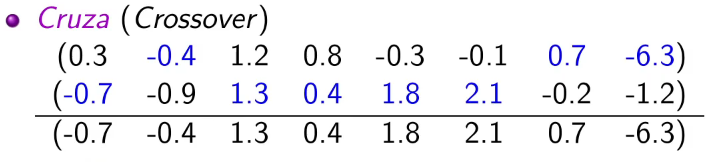
\includegraphics[width=0.9\linewidth]{images/cruza.png}
        \begin{quote}
        \caption{Ejemplo de una cruza entre dos codificaciones de redes neuronales
        \protect\cite{profa}}
        \end{quote}
        \label{fig:cruza}
        \end{figure}
    \item Cruza de un solo punto\\
        En esta operación tenemos dos cromosomas $A, B$ como entrada y dos cromosomas de salida $C_1, C_2$. Tomamos un punto $i$ aleatorio uniforme en los padres, al cual llamaremos punto cruza. En un hijo tomamos la información del padre del elemento $0$ hasta el $i$ y del padre $B$ del $i+1$ hasta el el ultimo, en el otro hijo invertimos el orden de los padres.
        
        En la figura $8$ se puede ver un ejemplo de la cruza de un solo punto.
        \begin{figure}[H]
        \centering
        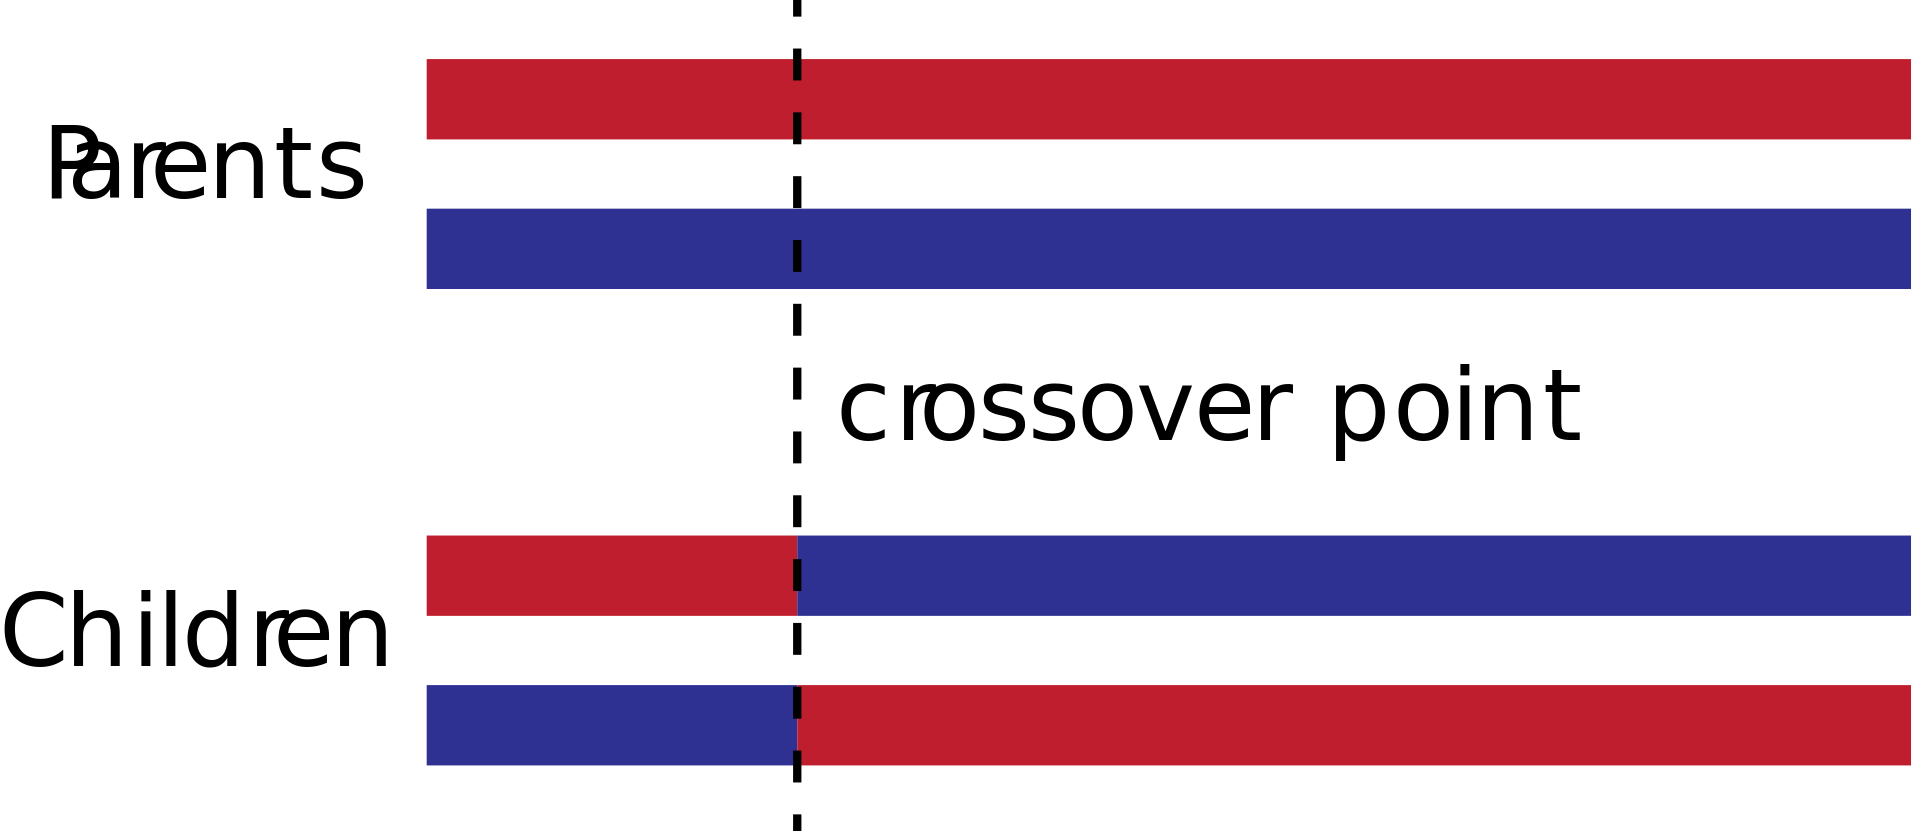
\includegraphics[width=0.9\linewidth]{images/OnePointCrossover.svg.png}
        \begin{quote}
        \caption{Cruza de un solo punto 
        \protect\cite{wiki_crossover}}
        \end{quote}
        \label{fig:mutacion}
        \end{figure}
    \item Cruza de $n$ puntos \\
    Similar a de un solo punto se seleccionan $n$ puntos y se hace una intercalación de elementos entre cada padre en los dos hijos.
    
    En la figura $8$ se puede ver un ejemplo de la cruza de dos puntos.
    \begin{figure}[H]
        \centering
        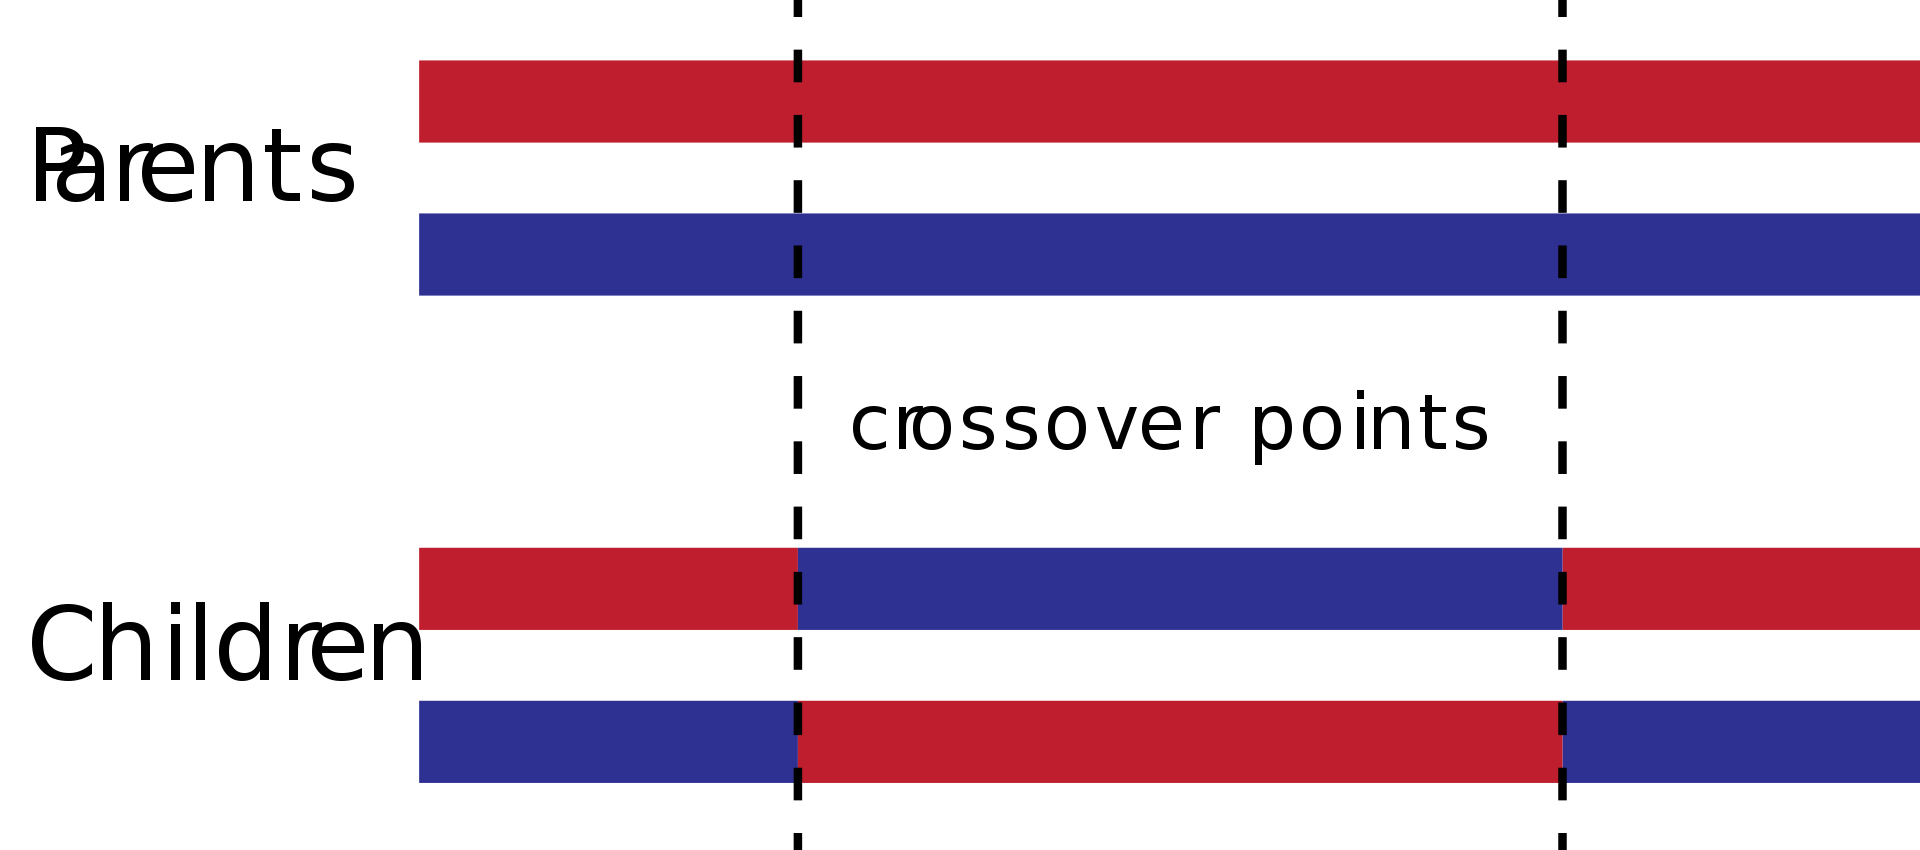
\includegraphics[width=0.9\linewidth]{images/TwoPointCrossover.svg.png}
        \begin{quote}
        \caption{Cruza de dos puntos
        \protect\cite{wiki_crossover}}
        \end{quote}
        \label{fig:mutacion}
    
    \end{figure}
        
\end{enumerate}






\section{Comparación entre AEB investigados}
Las estrategias de optimización de colonias de hormiga son bastante prometedoras cuando son aplicadas a la optimización de un solo objetivo, aunque en ocasiones ha sido superado por  algoritmos genéticos más comunes o estrategias de búsqueda más simples \cite{lopez2010automatic}. Los algoritmos de colonias de hormigas sufren del mismo problema que otros algoritmos genéticos y bio inspirados. Son eficaces, siempre y cuando se tenga suficiente poder de cómputo o tiempo disponible para resolver un problema dado. Un número suficiente de iteraciones deben cumplirse para la convergencia y el algoritmo puede ser extremadamente complejo de ejecutar \cite{fan2020review}. 

Como se mencionó anteriormente las ventajas más notables del algoritmo de banco de peces es que generalmente converge rápidamente a la solución óptima, que no suele ser sensible a las condiciones iniciales y que es fácil de implementar \cite{tian2009improved}. Entre las desventajas del algoritmo del banco de peces se encuentra que da malas soluciones a problemas no lineales y multimodales, que si los peces se mueven en dirección aleatoria no se aprovechará tiempo de cómputo para aproximar la solución de manera eficiente y que demasiados movimientos del banco pueden aumentar la complejidad del algoritmo y por lo tanto ralentizar la convergencia a la solución \cite{peng2018modification}.

Una de las grandes ventajas de los algoritmos de neuroevolución es que pueden ser aplicados para entrenar redes neuronales profundas, por lo cual es factible resolver problemas complejos con soluciones no lineales \cite{stanley2017welcoming,such2017deep}. Otra ventaja es que pueden entrenar redes neuronales más rápidamente que los métodos puramente matemáticos. Entre las desventajas está que debido a que en cada generación no se espera a que todos los individuos converjan hacia la solución óptima y a que las mutaciones son aleatorias en su naturaleza se puede desperdiciar tiempo de cómputo.

Notemos que los algoritmos de neuroevolución sí son capaces de resolver problemas no lineales y que pueden ser utilizados utilizan tecnología que se espera tenga un gran impacto en la realidad inmediata de la sociedad como podría ser la conducción autónoma \cite{goodfellow2016deep,stanley2017welcoming}. Además, los algoritmos de neuroevolución pueden ser aplicados a videojuegos logrando en algunos casos superar el rendimiento de los humanos \cite{mnih2015human}. Por estas razones es que elegimos trabajar con el algoritmo de neuroevolución en este proyecto y en particular aplicarlo a una versión del videojuego Flappy Bird.

\section{Aplicación de Neuroevolución a Flappy Bird}

\subsection{Descripción del juego}
\begin{figure}[ht]
    \centering
    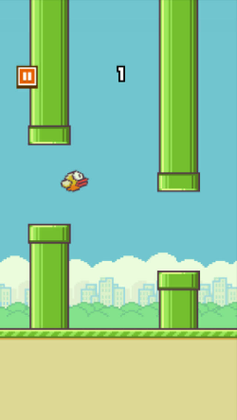
\includegraphics[width=0.55\linewidth]{images/Flappy_Bird_gameplay.png}
    \caption{Interfaz del juego de Flappy Bird.}
    \label{fig:gameplay}
\end{figure}

Flappy Bird (\cref{fig:gameplay}) es un juego para dispositivos móviles desarrollado por el artista y programador de videojuegos vietnamita Dong Nguyen, bajo su compañía de desarrollo de juegos dotGears. El jugador controla un pájaro que se desplaza hacia la derecha y que adicionalmente va cayendo debido a la gravedad. Periódicamente, el pájaro se va encontrando con pares de tuberías verdes con una apertura en el medio; el objetivo del juego es pasar por dicha apertura, evitando tocar las tuberías o el suelo. Para lograr esto, el usuario puede indicar al pájaro si aletear sus alas o no, lo cual inmediatamente le da una velocidad vertical positiva, que rápidamente empieza a decaer debido a la gravedad.

Debido a que la altura de la apertura de las tuberías cambia, el decidir cuándo aletear es un problema difícil que depende de diversos factores. Por lo tanto, se presta para ser resuelto utilizando algoritmos genéticos.

\subsection{Solución con redes neuronales y algoritmos evolutivos}
\begin{figure}[ht]
\centering
\begin{tikzpicture}[
	> = Stealth, semithick,
	plain/.style = {draw=none, fill=none,
		text width=7ex,  align=center},
	ec/.style = {draw=none},
	net/.style = {
		matrix of nodes,
		nodes={circle, draw, semithick, minimum size=7mm, inner sep=0mm},
		nodes in empty cells,
		column sep = 5mm, 
		row sep = 3mm
	},
	]
    	\matrix[net] (m)
    	{
    		|[plain]| Capa de entrada & |[plain]| Capa oculta    & |[plain]| Capa de salida  \\
    		|[ec]|                    &                          & |[ec]|                  \\
    		&                          & |[ec]|                  \\
    		|[ec]|                    &                          &                         \\
    		|[ec]|                    &                          & |[ec]|                  \\
    		&                          & |[ec]|                  \\
    		|[ec]|                    &                          & |[ec]|                  \\
    	};
    	\% inputs
    	\draw[<-] (m-3-1.west) -- node[above] {$\Delta x$} +(-10mm,0);
    	\draw[<-] (m-6-1.west) -- node[above] {$\Delta y$} +(-10mm,0);
    	\foreach \j in {3,6}
    	{
    		\foreach \k in {2,...,7} \draw[->] (m-\j-1) -- (m-\k-2);
    	}
    	\foreach \j in {2,...,7}
    	{
    		\foreach \k in {4} \draw[->] (m-\j-2) -- (m-\k-3);
    	}
    	\draw[->] (m-4-3.east) -- node[above] {¿Aletear?} +(15mm,0);
    \end{tikzpicture}
    \caption{Diagrama de la red neuronal. $\Delta x$ y $\Delta y$ representan la distancia horizontal y vertical del pájaro a la apertura, respectivamente.}
    \label{fig:red}
\end{figure}

Para modelar la inteligencia artifical de un pájaro, utilizamos una red neuronal con una capa de entrada, una capa oculta, y una capa de salida. La descripción de cada una de estas capas es la siguiente:
\begin{itemize}
    \item Capa de entrada: Dos neuronas con función de activación sigmoide, que toman como argumento la distancia vertical y horizontal del pájaro al centro de la apertura entre las tuberías.
    \item Capa oculta: Seis neuronas con función de activación sigmoide, completamente conectadas a la capa anterior.
    \item Capa de salida: Una neurona conectada a la capa anterior. Regresa verdadero si su valor es mayor a 0.5, y falso en otro caso.
\end{itemize}
El diagrama puede verse en la \cref{fig:red}.

Por otro lado, para entrenar nuestro algoritmo, seguimos los siguientes pasos:
\begin{enumerate}
	\item Creamos una población inicial de $n$ pájaros con una red neuronal artificial aleatoria para cada pájaro
	\item Dejamos que cada pájaro juegue.
	\item Terminamos la simulación cuando todos los pájaros estén muertos, o se alcance el tiempo máximo.
    \item Producimos la siguiente generación.
\end{enumerate}

Evidentemente, el paso más importante de este método es la adecuada selección de los individuos para obtener la siguiente generación. Como se mencionó en secciones anteriores, cada nueva población está compuesta de tres grupos distintos: 
\begin{itemize}
    \item $E$: individuos élite, que pasan su genoma sin ningún cambio.
    \item $H$: hijos de dos individuos de la población anterior.
    \item $N$: individuos ``normales'', seleccionados aleatoriamente de la generación anterior.
\end{itemize}
Para escoger los pares de padres de los individuos de la clase $H$, utilizamos dos algoritmos diferentes de selección
\begin{itemize}
    \item Selección aleatoria basada en \textit{fitness} (ruleta)
    \item Selección por torneo
\end{itemize}
Adicionalmente, mutamos los individuos de las clases $H$ y $N$ escogiendo pesos aleatorios y sumándoles ruido gaussiano de la forma con media 0 y varianza 1. Para determinar cuántos pesos mutamos, definimos una tasa de mutación $m$, la cual determinará la fracción total del genoma a mutar. Es importante notar que $m$ \textbf{no} representa el porcentaje de individuos; por ejemplo, si $m=0.01$ significa que el 1\% del genoma colectivo sufrirá mutaciones, antes de ser distribuido a cada uno de los individuos. Por lo tanto, puede haber algunos pájaros que después de nacer no muten en lo absoluto, y otros que lo hagan bastante.

\section{Implementación}
\subsection{Elementos}
En esta sección damos una breve descripción de las partes más importantes de la implementación en Python de nuestro sistema. Invitamos a revisar el documento disponible en el repositorio del proyecto\footnote{\url{https://github.com/patoba/LCD-CC-2020-I}} si se desea una documentación detallada.

\subsubsection{Redes}
Cada capa de las redes neuronales es un objeto de tipo \texttt{Layer}, con los siguientes atributos:
\begin{itemize}
    \item \texttt{W}: Arreglo de tamaño $m\times n$, donde $m$ es el número de neuronas en la capa anterior, y $n$ el de la capa actual. Este representa los pesos de la capa.
    \item \texttt{b}: Vector de tamaño $n$, equivalente a el \textit{bias} de cada neurona.
    \item \texttt{f}: Función de activación de todas las neuronas de la capa.
\end{itemize}
Para evaluar un vector de entrada $v$ en alguna capa, simplemente calculamos $\texttt{W}\cdot v + \texttt{b}$, y aplicamos \texttt{f} a cada uno de los elementos del vector resultante.

Una red neuronal es simplemente un objeto de tipo \texttt{NeuralNet} con dos atributos: \texttt{layers}, una lista de objetos de tipo \texttt{Layer}, y \texttt{f}, la función de activación de la última capa. 

Para evaluar un vector a través de esta red, lo evaluamos en cada una de sus capas de manera secuencial, y aplicamos \texttt{f} al último resultado. Recordemos que en nuestro caso la última capa consiste de una sola neurona, y \texttt{f} es la función definida por partes:
\begin{equation*}
    f(x)=
    \begin{cases}
     \text{Verdadero} & x < 0.5\\
     \text{Falso} & x\geq 0.5
    \end{cases}
\end{equation*}

Un par de métodos asociados a la clase \texttt{NeuralNet} y que usaremos de manera extensa son \texttt{encode} y \texttt{decode}. Como indican sus nombres, estos se encargan de codificar y decodificar las propiedades de la red, usando el método descrito en el \cref{sec:codificacion}.

\subsubsection{Pájaros}
Cada pájaro está descrito por un objeto de clase \texttt{Bird}. Aparte de guardar los parámetros físicos necesarios para su simulación (posición, velocidad, aceleración de la gravedad, etc.), tiene los siguientes campos:
\begin{itemize}
    \item \texttt{alive}: Si está vivo o no.
    \item \texttt{fitness}: Aptitud actual; cuando el pájaro nace es cero, y va aumentando conforme el pájaro se mueve en el tiempo (más detalles en una sección posterior).
    \item \texttt{network}: Objeto de tipo \texttt{NeuralNet}.
\end{itemize}
El pájaro decide si aletear o no con base en la salida de su red.

\subsubsection{Tuberías}
Las tuberías son representadas con la clase \texttt{Pipe}. Para simplificar las entradas a la red neuronal de los pájaros, hacemos que las tuberías sean las que se desplazan horizontalmente, mientras que los pájaros están fijos en $x=0$. Por lo tanto, cada tubería tiene como atributos su posición y velocidad horizontales.

\subsubsection{Mundo}
Representamos el mundo en el que yacen los pájaros y las tuberías con un objeto de tipo \texttt{World}. Este se encarga de mover a todos los elementos en cada instante de tiempo, y de revisar si algún pájaro chocó contra una tubería o contra el suelo, matándolo en caso afirmativo. Adicionalmente, como puede haber múltiples tuberías en pantalla, y dado que estas son destruidas y creadas cuando se salen de los límites del mundo, el objeto \texttt{World} informa a los pájaros cuál es la tubería más cercana, para que puedan decidir si aletear o no. Finalmente, después de haber actualizado todos los objetos, recompensa a los pájaros que siguen vivos sumando al atributo \texttt{fitness} de cada uno un valor $r_a$, con una bonificación adicional $r_p$ si lograron pasar una tubería.

\subsection{Simulación}
La evolución de una generación de individuos puede describirse de la siguiente manera:

\begin{algorithm}
\caption{Bucle principal de un mundo.}
\label{alg:mundo}
\begin{algorithmic}[]
\While{algún pájaro esté vivo o $n<\texttt{pasos\_máximos}$}
    \State $\texttt{mover\_pájaros}()$
    \State $\texttt{mover\_tuberías}()$
    \For{$p\in \texttt{pájaros}$}
        \For{$t\in \texttt{tuberías}$}
            \If{\texttt{colisión(p,t)}} \Comment{Si $p$ y $t$ chocan}
                \State $\texttt{p.alive} \gets \texttt{Falso}$ \Comment{Matamos al pájaro}
            \EndIf
        \EndFor
    \EndFor
    
    \For{$p\in \texttt{pájaros}$} \Comment{Recompensas}
        \If{$p$ está vivo}
            \State $\texttt{p.fitness}\gets \texttt{p.fitness} + r_a$ 
            \If{$p$ pasó tubería}
                \State $\texttt{p.fitness}\gets \texttt{p.fitness} + r_p$ \
            \EndIf
        \EndIf
    \EndFor
    \State $n\gets n+1$
\EndWhile
\end{algorithmic}
\end{algorithm}
Donde:
\begin{itemize}
    \item $n$: Contador de pasos. El algoritmo acaba cuando todos los pájaros mueren o $n$ es mayor a \texttt{pasos\_máximos}.
    \item $\texttt{colisión}(p,t)$: Función que revisa si el pájaro $p$ y la tubería $t$ chocaron. Como el primero es un círculo y el segundo un rectángulo, podemos usar geometría para determinar esto.
    \item $r_a$: Recompensa por mantenerse vivo una unidad de tiempo.
    \item $r_p$: Recompensa por cruzar una tubería.
\end{itemize}

Al final de la simulación, cada pájaro tendrá en su atributo \texttt{fitness} la \textit{fitness} que alcanzó, con la cual podemos crear una nueva generación.

\subsection{Algoritmo genético}
Como mencionamos anteriormente, para producir una nueva generación, debemos de seleccionar tres grupos de individuos diferentes: élites ($E$), normales ($N$) e hijos ($H$). A continuación, describimos cómo escoger cada uno:

\begin{itemize}
    \item Élites: Dado que por definición los individuos de este grupo son los mejores de la generación, simplemente ordenamos los pájaros por \textit{fitness}, y escogemos los $E$ mejores.
    \item Normales: Tan sólo tomamos $N$ pájaros de manera aleatoria.
    \item: Para escoger a cada par de padres, utilizamos uno de los métodos de selección posibles: aleatoria basada en \textit{fitness} (también conocida como ruleta) y por torneos. Escogemos $H/2$ pares diferentes (ya que bajo \textit{crossover} de un solo punto cada par de padres produce un hijo). Adicionalmente, permitimos que los padres estén presentes en más de una pareja.

    Una vez hecho esto, hacemos \textit{crossover} sobre cada pareja.

\end{itemize}

\subsection{Concurrencia}\label{sec:concurrencia}
Naturalmente, el simular muchas generaciones de manera secuencial es un proceso muy tardado, ya que hay que actualizar cada objeto en el mundo. Sin embargo, gracias a la manera en que estructuramos nuestro sistema, el diseñar una implementación paralela es una tarea relativamente sencilla.

Si queremos simular una generación con $n$ pájaros, y asumiendo que nuestro sistema puede ejecutar $p$ procesos en paralelo, tenemos dos opciones:
\begin{enumerate}
    \item Creamos $p$ mundos, y en cada uno de ellos cargamos $\lfloor n/p\rfloor$ pájaros. Posteriormente, asignamos cada mundo a un proceso diferente y los ejecutamos paralelamente.
    \item Creamos $n$ mundos, y en cada uno ponemos un solo pájaro. Ejecutamos los primeros $p$ mundos de manera paralela, luego los siguientes $p$, y así sucesivamente hasta agotar los mundos disponibles.
\end{enumerate}
En la siguiente sección veremos la diferencia entre estas dos implementaciones, y cuál es más adecuada para nuestro problema. 

Afortunadamente, ambos métodos pueden implementarse utilizando la estructura de datos \texttt{Pool} del módulo \texttt{multiprocessing}. Para hacerlo, recolectamos todos los mundos a simular en una lista (llámese \texttt{worlds}) y ejecutamos \texttt{pool.map(worlds, play)}, donde \texttt{play} es un método de la clase \texttt{World} que simula el mundo siguiendo los pasos descritos en el \cref{alg:mundo} y regresa los pájaros una vez terminado. 

El objeto \texttt{pool} es una mezcla entre los conceptos familiares de cola y \textit{mutex}. Como primer paso, asigna a cada proceso uno de los objetos a analizar (en este caso, nuestros mundos), después de lo cual los procesos ejecutan la función indicada (\texttt{play}) sobre ellos. Una vez que todos los procesos hayan terminado (indicado por un \textit{mutex}), colecta los resultados y vuelve a asignar a cada proceso un objeto nuevo.

Otro beneficio importante de usar \texttt{Pool} es que el algoritmo puede ser escalado a más pájaros o procesos sin necesidad de hacer ningún cambio en el código.

\section{Resultados}
\subsection{Método de evaluación}
Antes que nada, hay que determinar el método de evaluación a usar. Dado que procesos como selección o mutación son inherentemente aleatorios (así como las poblaciones iniciales), existe la posibilidad de que algunos individuos de las primeras generaciones presenten un \textit{fitness} más alto de lo esperado. Esto nos impide considerar el \textit{fitness} máximo de una generación como métrica, ya que puede no ser representativo de la población completa. Adicionalmente, dado que estos individuos sobrevivirán mucho más que sus hermanos (al tener un \textit{fitness} mayor), el tiempo de ejecución de una generación entera tampoco es una buena medida de eficiencia.

A pesar de estas diferencias aleatorias, entre más vayan evolucionando las poblaciones, más irá aumentando el \textit{fitness} \textbf{promedio} de cada generación, ya que los individuos menos aptos serán reemplazados por unos más especializados. Por lo tanto, proponemos usar como métrica de evaluación el tiempo que tarda en alcanzar una población un cierto \textit{fitness}. De esta manera, garantizamos que se estén considerando las propiedades de todos los individuos.

\subsection{Parámetros predeterminados}
En los apartados siguientes, empezaremos haciendo una comparación entre distintas implementaciones concurrentes de nuestro algoritmo, para lo cual necesitamos ejecutarlo. Por lo tanto, establecemos los siguientes parámetros base:
\begin{itemize}
    \item Total de pájaros: 40
    \item Número de procesos (a menos que se especifique lo contrario): 4
    \item Elitismo : 10\%
    \item Tasa de \textit{crossover}: 80\%
    \item Tasa de mutación: 3\%
    \item Método de seleción: Torneo
    \item Participantes en torneo: 8
\end{itemize}

Incluimos estos parámetros aquí para tener un estándar para comparar los distintos resultados. 

\subsection{Distribución de trabajo}
\begin{figure}[hb]
\centering
    \begin{subfigure}{\linewidth}
        \centering
        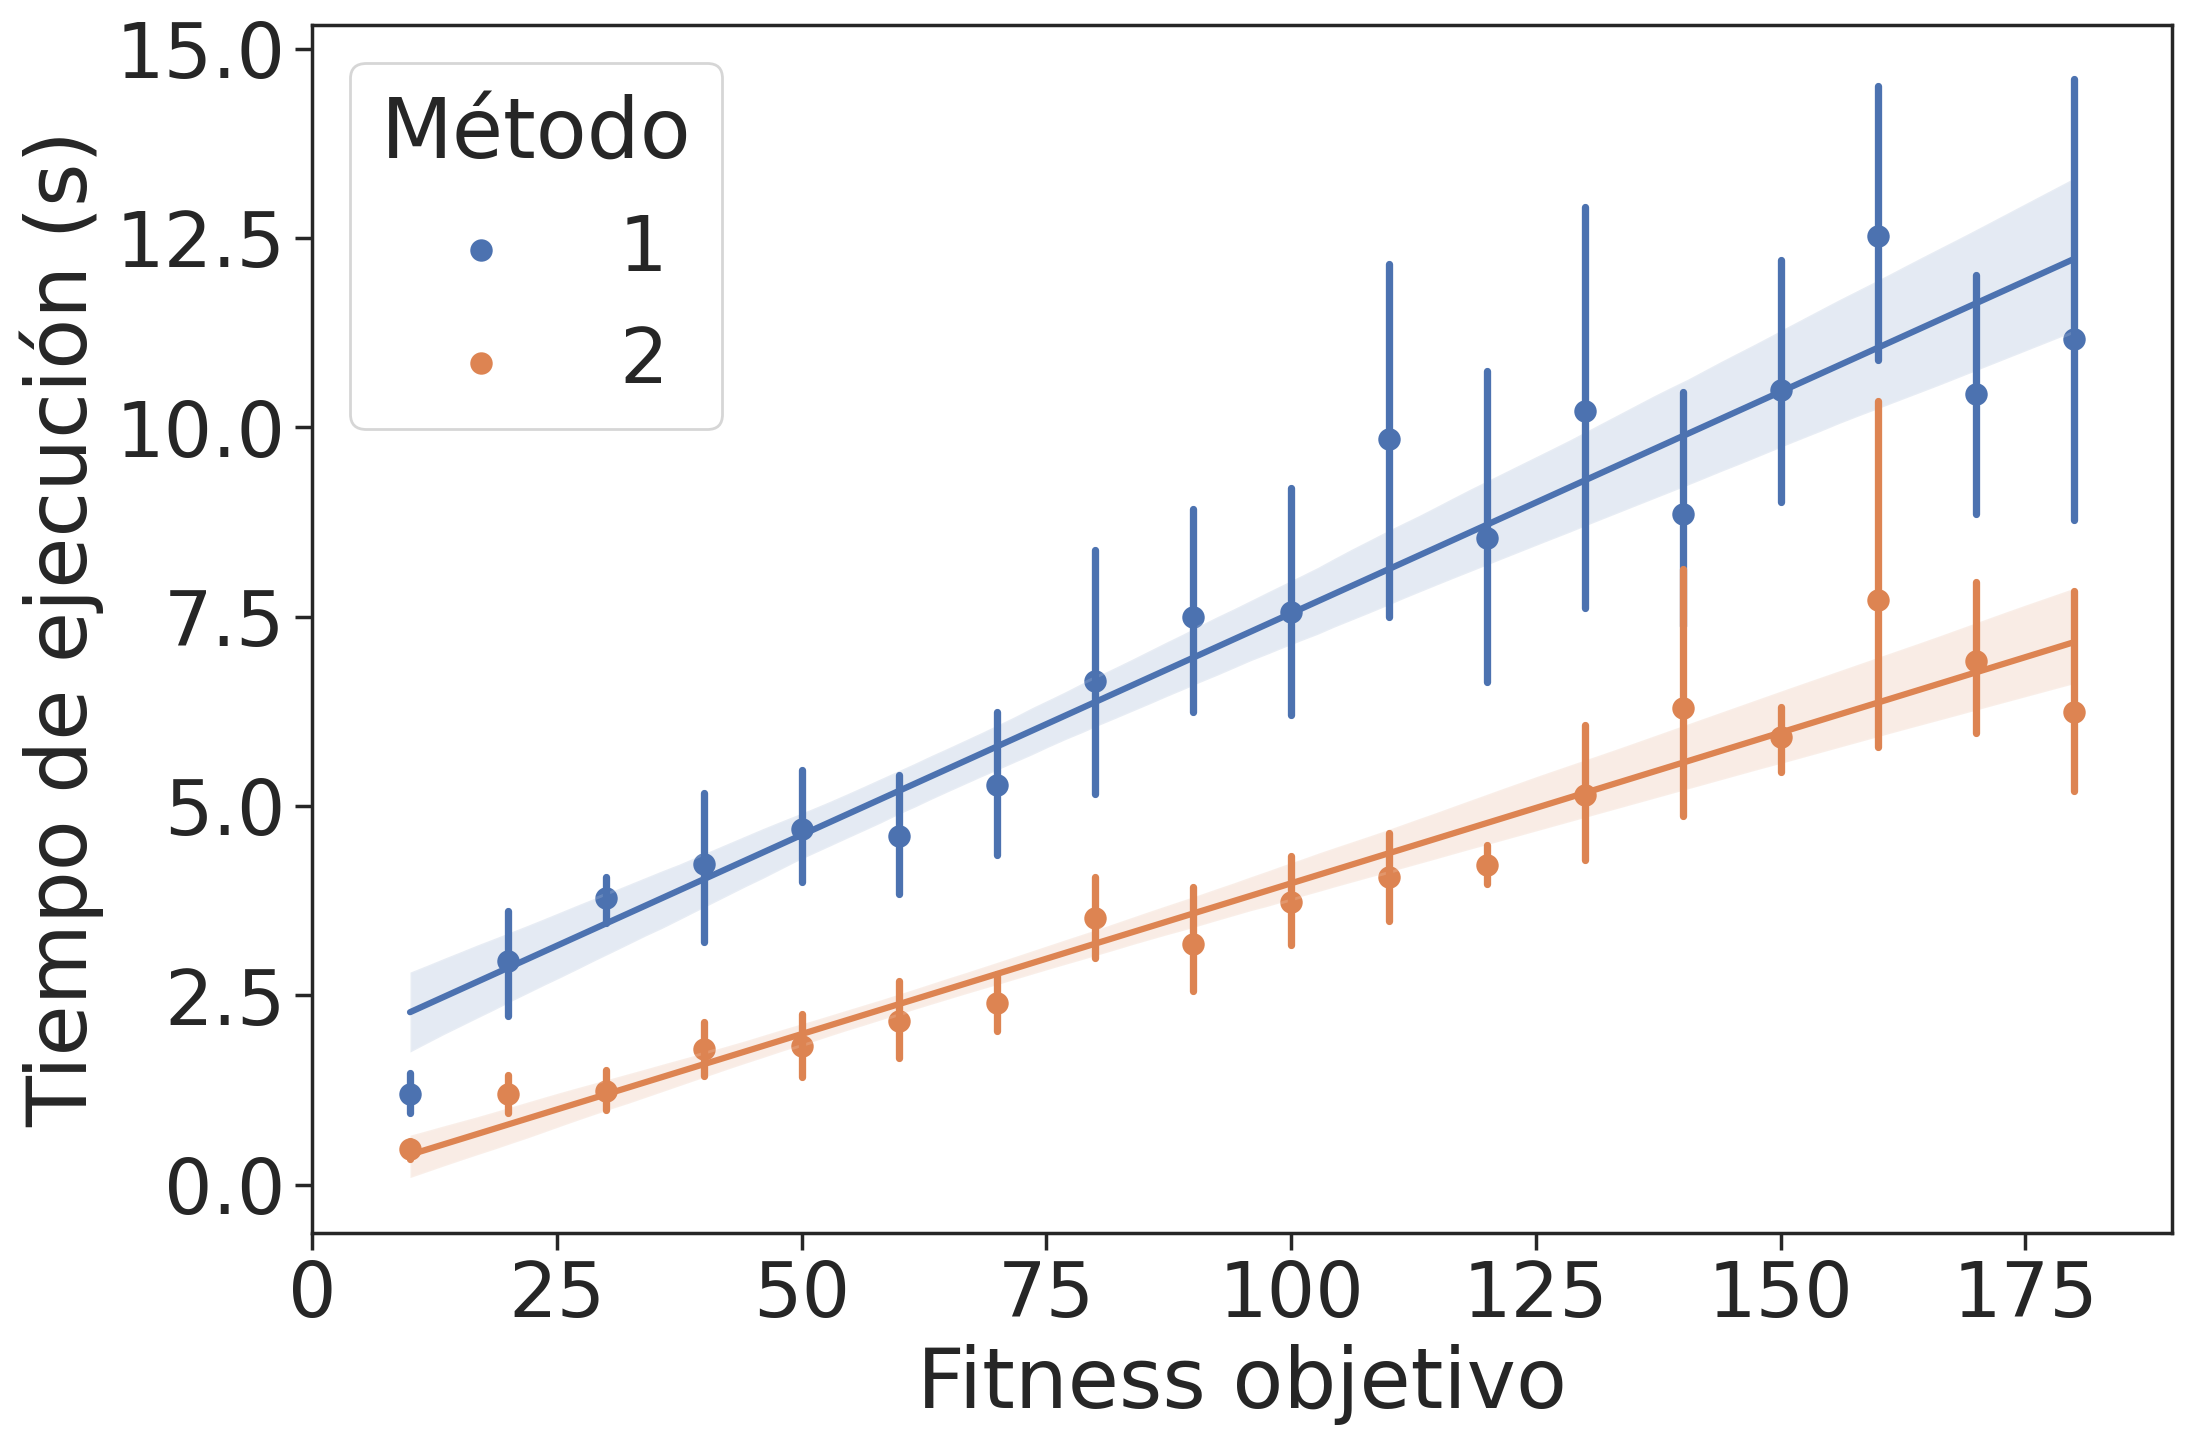
\includegraphics[width=0.9\linewidth]{eval_metodos.png}
        \caption{Tiempos de ejecución.}
        \label{fig:eval_metodos}
    \end{subfigure}%
    ~\\\vspace{12pt}
    \begin{subfigure}{\linewidth}
        \centering
        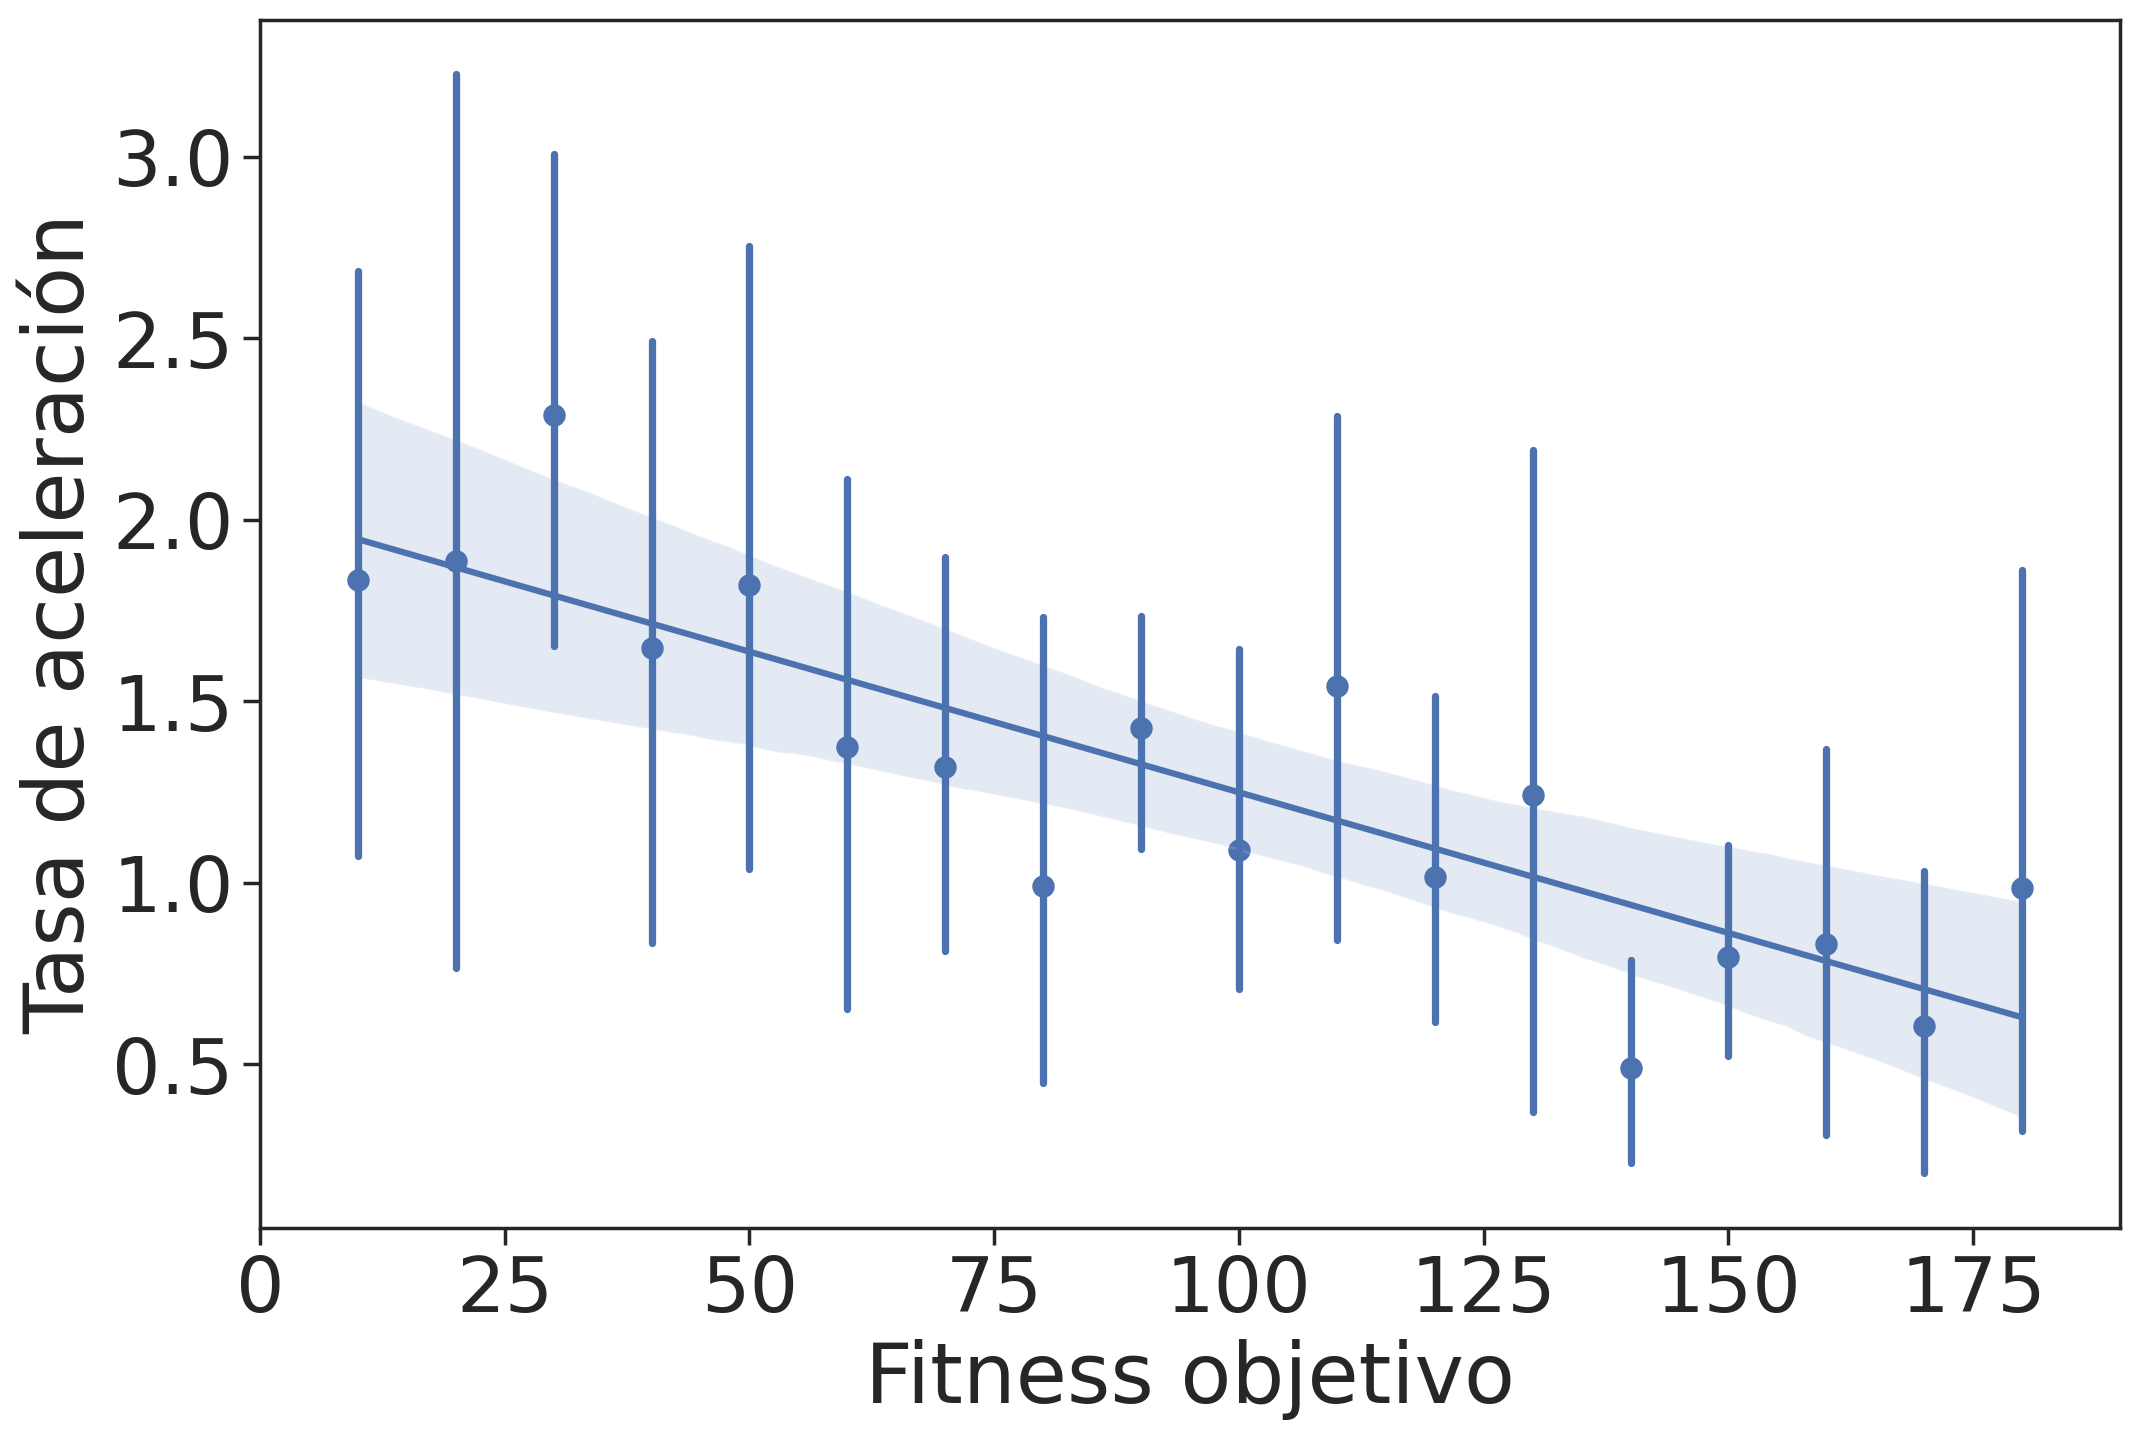
\includegraphics[width=0.9\linewidth]{acel_metodos.png}
        \caption{Tasa de aceleración ($\frac{\text{tiempo método 1}}{\text{tiempo método 2}}-1$)}
        \label{fig:acel_metodos}
    \end{subfigure}%  
    \caption{Tiempos de ejecución y tasas de aceleración promediadas sobre $n=7$ ejecuciones para distintos métodos. Se muestran ajustes lineales con intervalos de confianza del 95\%.}
    \label{metodos}
\end{figure}
Comparamos los dos métodos de simulación mencionados en el \cref{sec:concurrencia}; como recordatorio (tomando nuestra población de 40 pájaros y 4 procesos) estos son:
\begin{itemize}
    \item Método 1: Crear 4 mundos de 10 pájaros cada uno, y ejecutar cada mundo de manera paralela.
    \item Método 2: Crear 40 mundos de 1 pájaro cada uno y ejecutar mundos de cuatro en cuatro de manera paralela.
\end{itemize}
Los resultados pueden verse en la \cref{metodos}. 

Como puede notarse, el método dos es mucho más rápido que el uno, con una tasa de aceleración de hasta 4 veces en comparación. Esto se debe a que los procesos del método 1 deben de esperar hasta que todos los pájaros de los demás procesos acaben de ejecutarse. Por lo tanto, si un proceso termina muy rápido (debido a que sus pájaros tenían una \textit{fitness} muy baja) tiene que estar en espera de los demás procesos. Esto no ocurre con el segundo método, ya que al ser mundos con un sólo pájaro, el tiempo que están en espera los procesos es mucho menor.

Es interesante ver que la tasa de aceleración decrece conforme va aumentando el \textit{fitness} objetivo. Podemos explicar esto recordando que un \textit{fitness} promedio mayor inherentemente requiere de más generaciones, lo cual a su vez implica que cada vez habrá menos diferencias entre cada uno de los mundos asignados a los distintos procesos. Por lo tanto, cada proceso pasará menos tiempo en espera de que acaben los demás, ya que sus poblaciones serán aproximadamente equivalentes. A pesar de esto, el segundo método tiene un desempeño hasta dos veces mejor que el primero, por lo cual será el que utilizaremos en todos los análisis posteriores.

\subsection{Concurrencia}
\begin{figure}[ht]
\centering
    \begin{subfigure}{\linewidth}
        \centering
        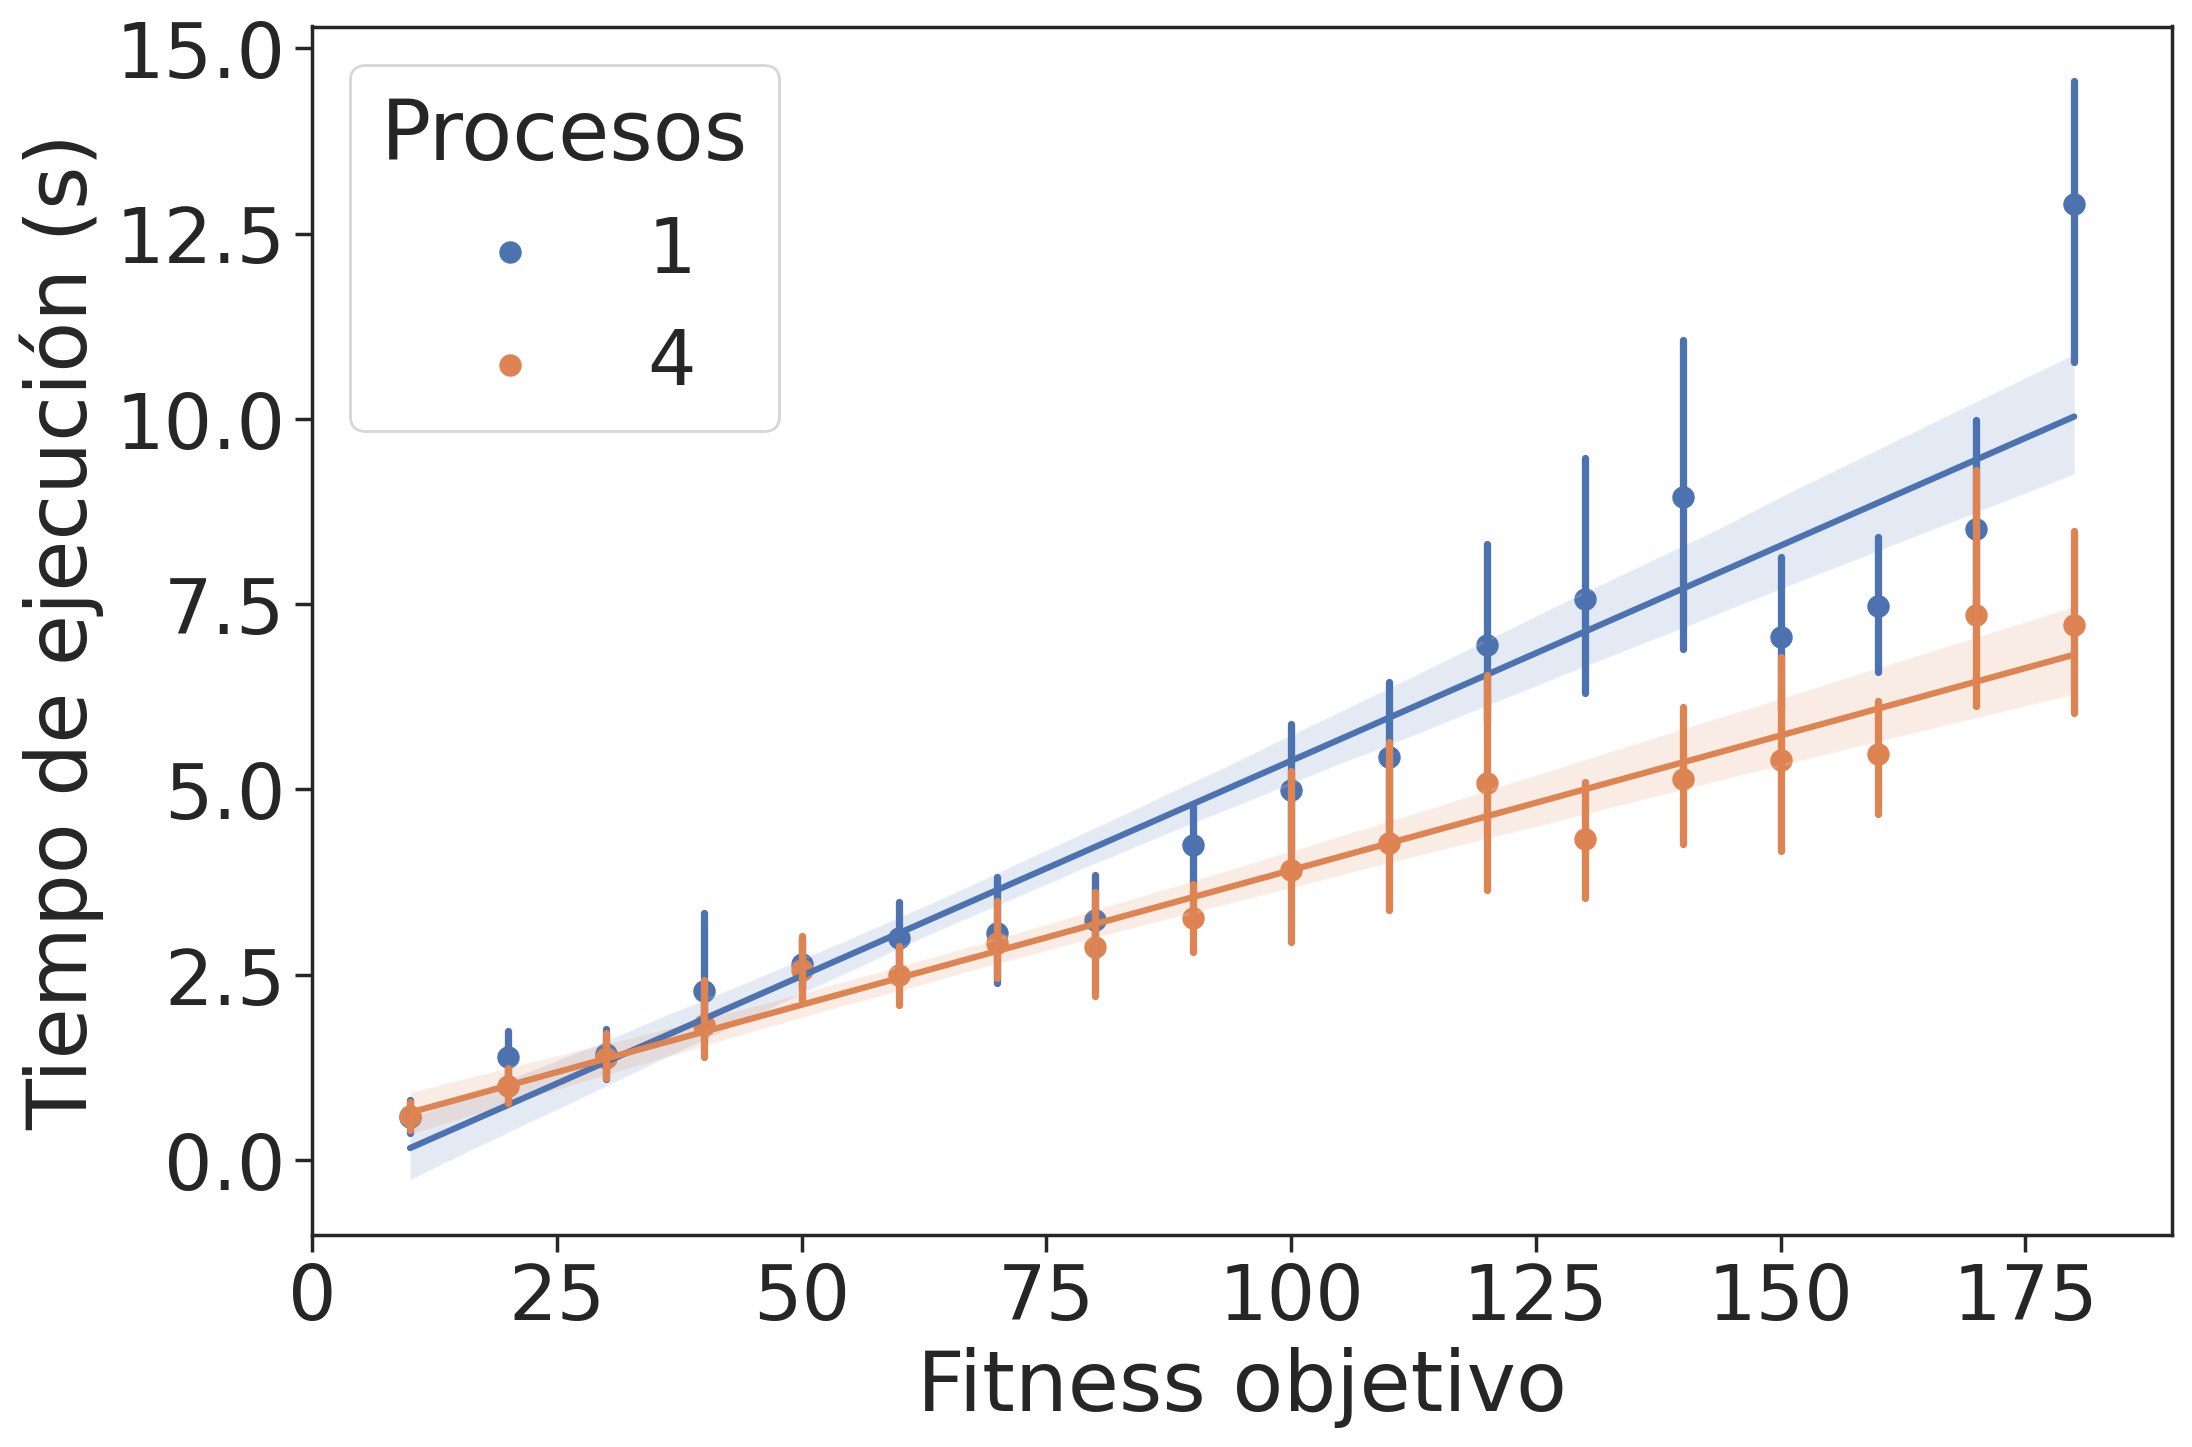
\includegraphics[width=0.9\linewidth]{eval_procesos.png}
        \caption{Tiempos de ejecución.}
        \label{fig:eval_procesos}
    \end{subfigure}%
    ~\\\vspace{12pt}
    \begin{subfigure}{\linewidth}
        \centering
        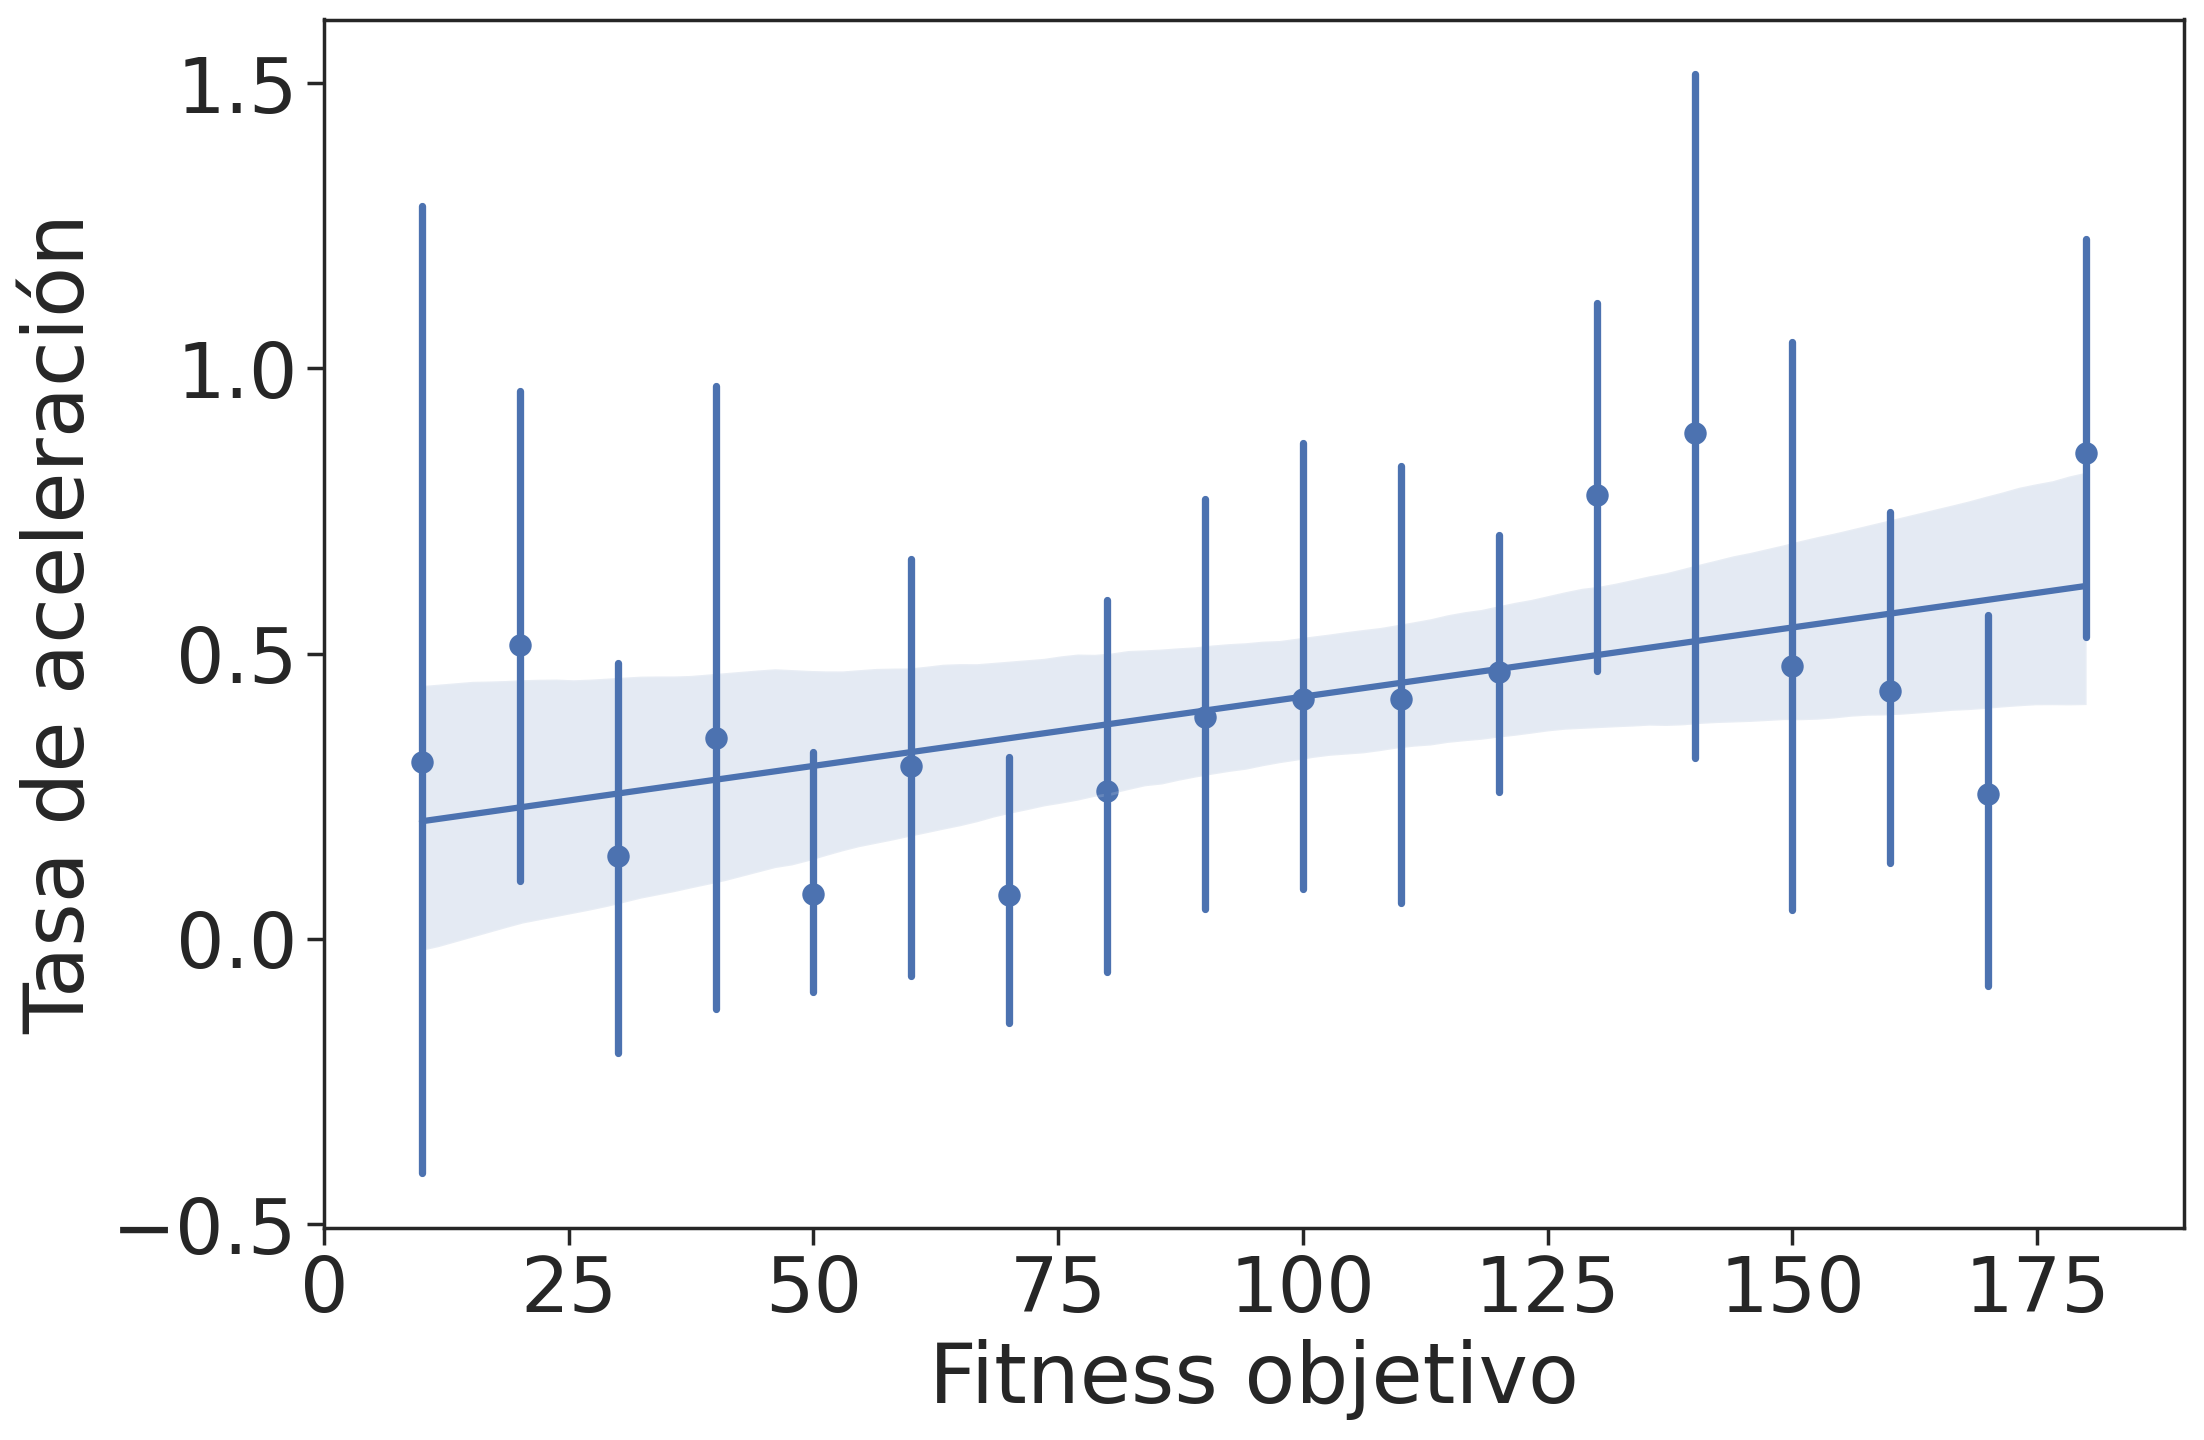
\includegraphics[width=0.9\linewidth]{acel_procesos.png}
        \caption{Tasa de aceleración ($\frac{\text{tiempo 1 proceso}}{\text{tiempo 4 procesos}}-1$)}
        \label{fig:acel_procesos}
    \end{subfigure}%  
    \caption{Tiempos de ejecución y tasas de aceleración promediadas sobre $n=7$ ejecuciones para distinto número de procesos.}
    \label{procesos}
\end{figure}
Una vez determinado la mejor forma de distribución de trabajo, el siguiente paso lógico es observar qué ocurre si utilizamos un número distinto de procesos. Los resultados para un proceso secuencial y cuatro procesos ejecutados de manera concurrente pueden verse en la \cref{procesos}. 

Si bien para las primeras generaciones prácticamente no hay diferencia (ya que para este punto los tiempos de ejecución son muy pequeños para aprovecharse de la concurrencia) conforme va incrementando el objetivo se va apreciando una diferencia cada vez más significativa entre los tiempos. El hecho de que la recta en la \cref{fig:acel_procesos} sea creciente sirve para confirmar este hecho, lo cual nos dice que nuestra implementación efectivamente se beneficia de la ejecución paralela, con tasas de aceleración de casi el 100\% para los \textit{fitness} objetivos más grandes.

\subsection{Métodos de selección}
\begin{figure}[ht]
    \centering
    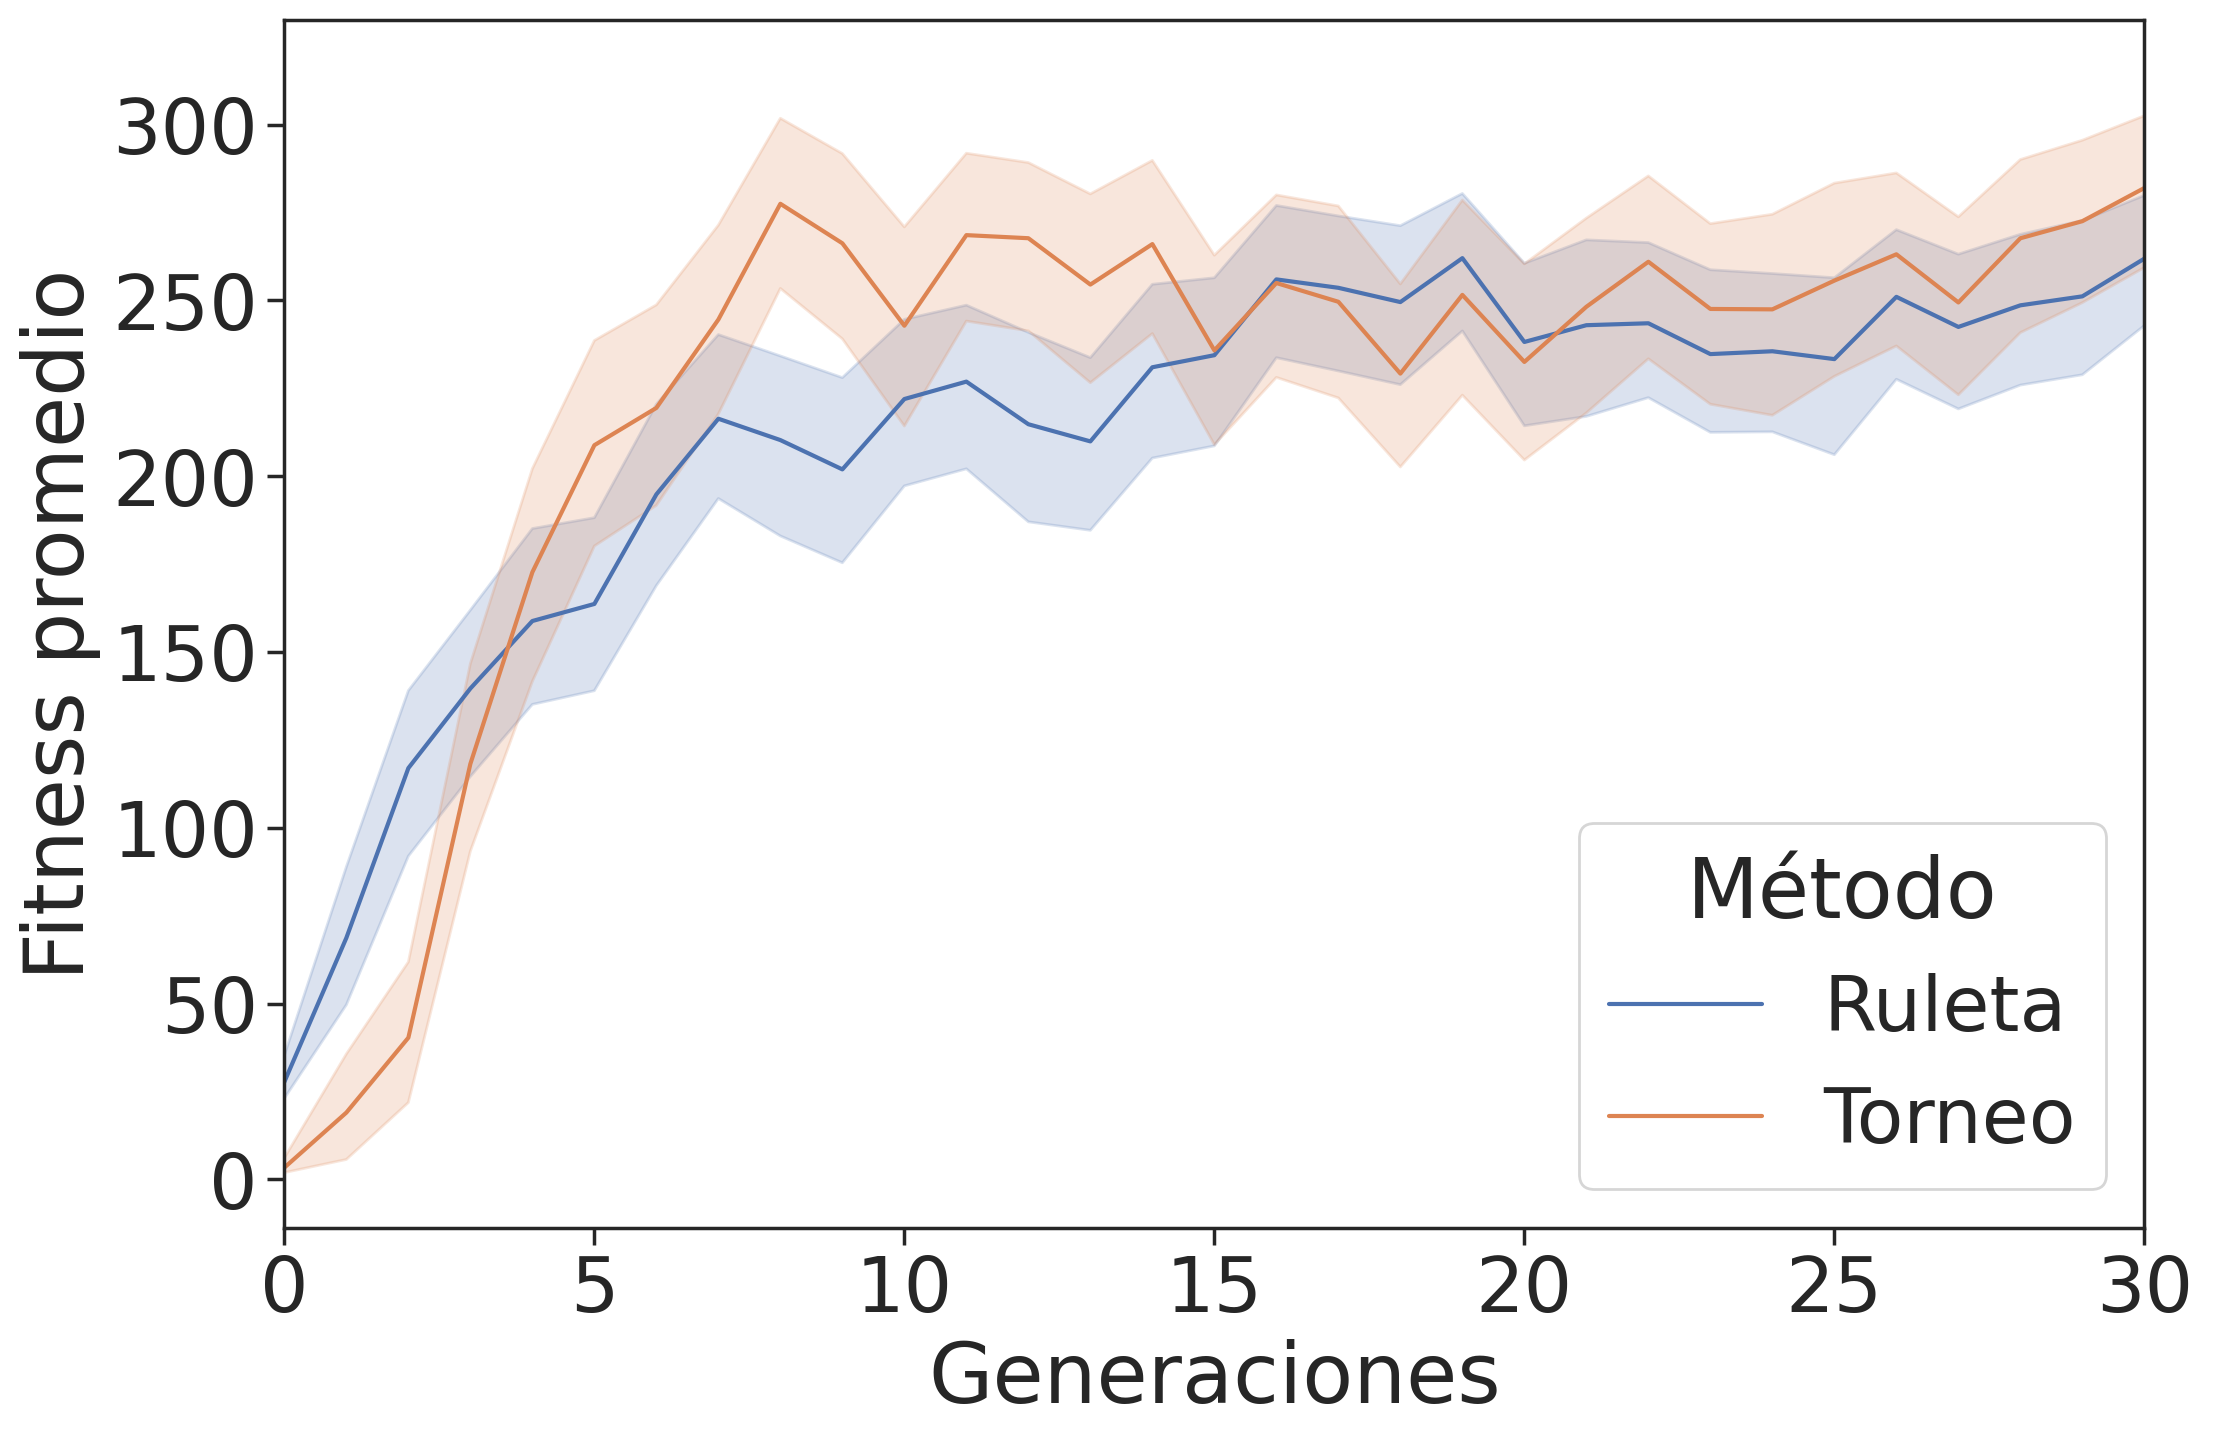
\includegraphics[width=0.9\linewidth]{eval_seleccion.png}
    \caption{Fitness por generación para ambos métodos de selección.}
    \label{fig:eval_seleccion}
\end{figure}

Como mencionamos previamente, tenemos la posibilidad de usar dos métodos diferentes al momento de seleccionar los padres. En la \cref{fig:eval_seleccion}, representamos el \textit{fitness} promedio de cada generación con ambos métodos. 

Podemos notar que el método de torneo converge un poco más rápido que el de ruleta. Adicionalmente, presenta ``picos'' menos pronunciados en su curva. Estos picos se deben a ruido estocástico producido por mutaciones y reproducción, y son fundamentales para mantener una población diversa. Sin embargo, no deben de ser muy grandes, ya que es posible que el \textit{fitness} decrezca de manera inesperada. El algoritmo de torneo evita este fenómeno comparando múltiples individuos entre sí, lo cual hace que sea menos probable escoger uno con un \textit{fitness} bajo. En el apartado siguiente, discutimos los efectos que tiene el número de individuos sobre el desempeño de las poblaciones.

\subsection{Participantes}
\begin{figure}[ht]
    \centering
    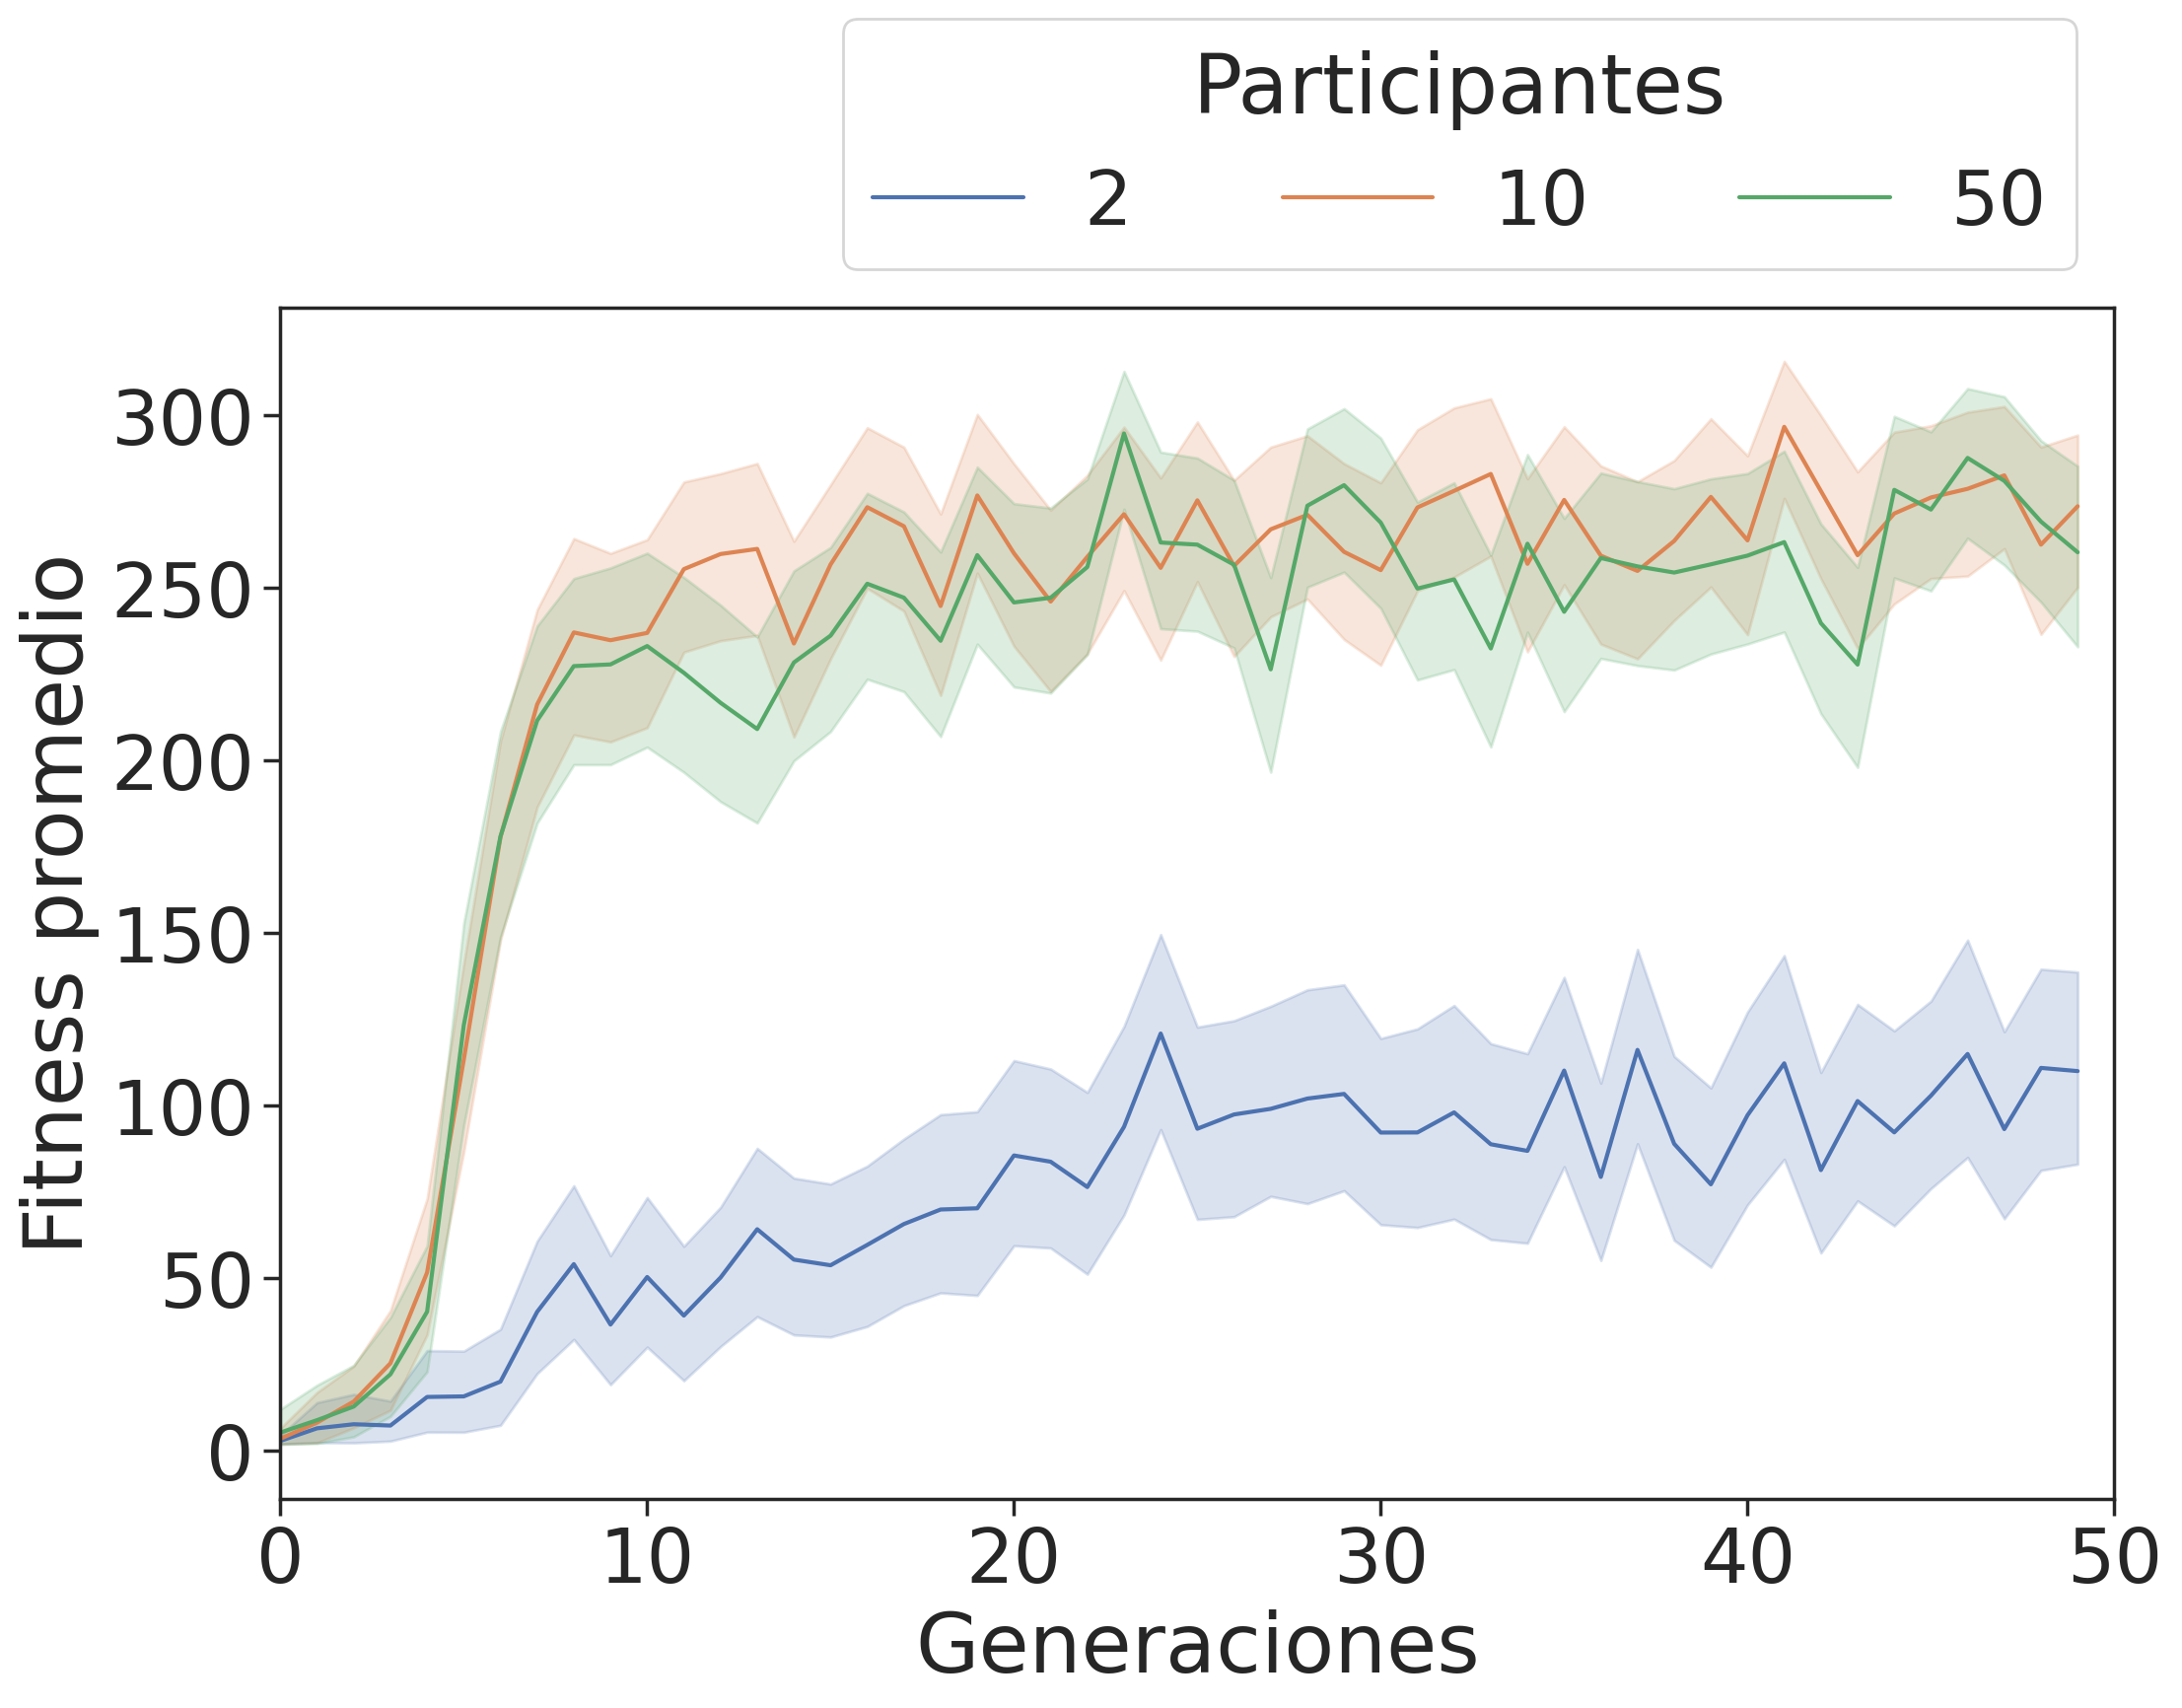
\includegraphics[width=0.9\linewidth]{eval_participantes.png}
    \caption{Fitness por generación para distinta cantidad de participantes..}
    \label{fig:eval_participantes}
\end{figure}

Para el método de selección por torneo, el número de participantes nos ayuda a ajustar la llamada \textit{presión de selección} \cite{Miller1995GeneticAT}. La razón es que con torneos más grandes, los individuos débiles tienen menos probabilidad de ser seleccionados, ya que si un individuo débil es escogido para participar en un torneo, es más probable que un individuo fuerte se encuentre en el mismo torneo. 

\begin{figure*}[t]
    \centering
    \begin{subfigure}[t]{0.25\linewidth}
        \centering
        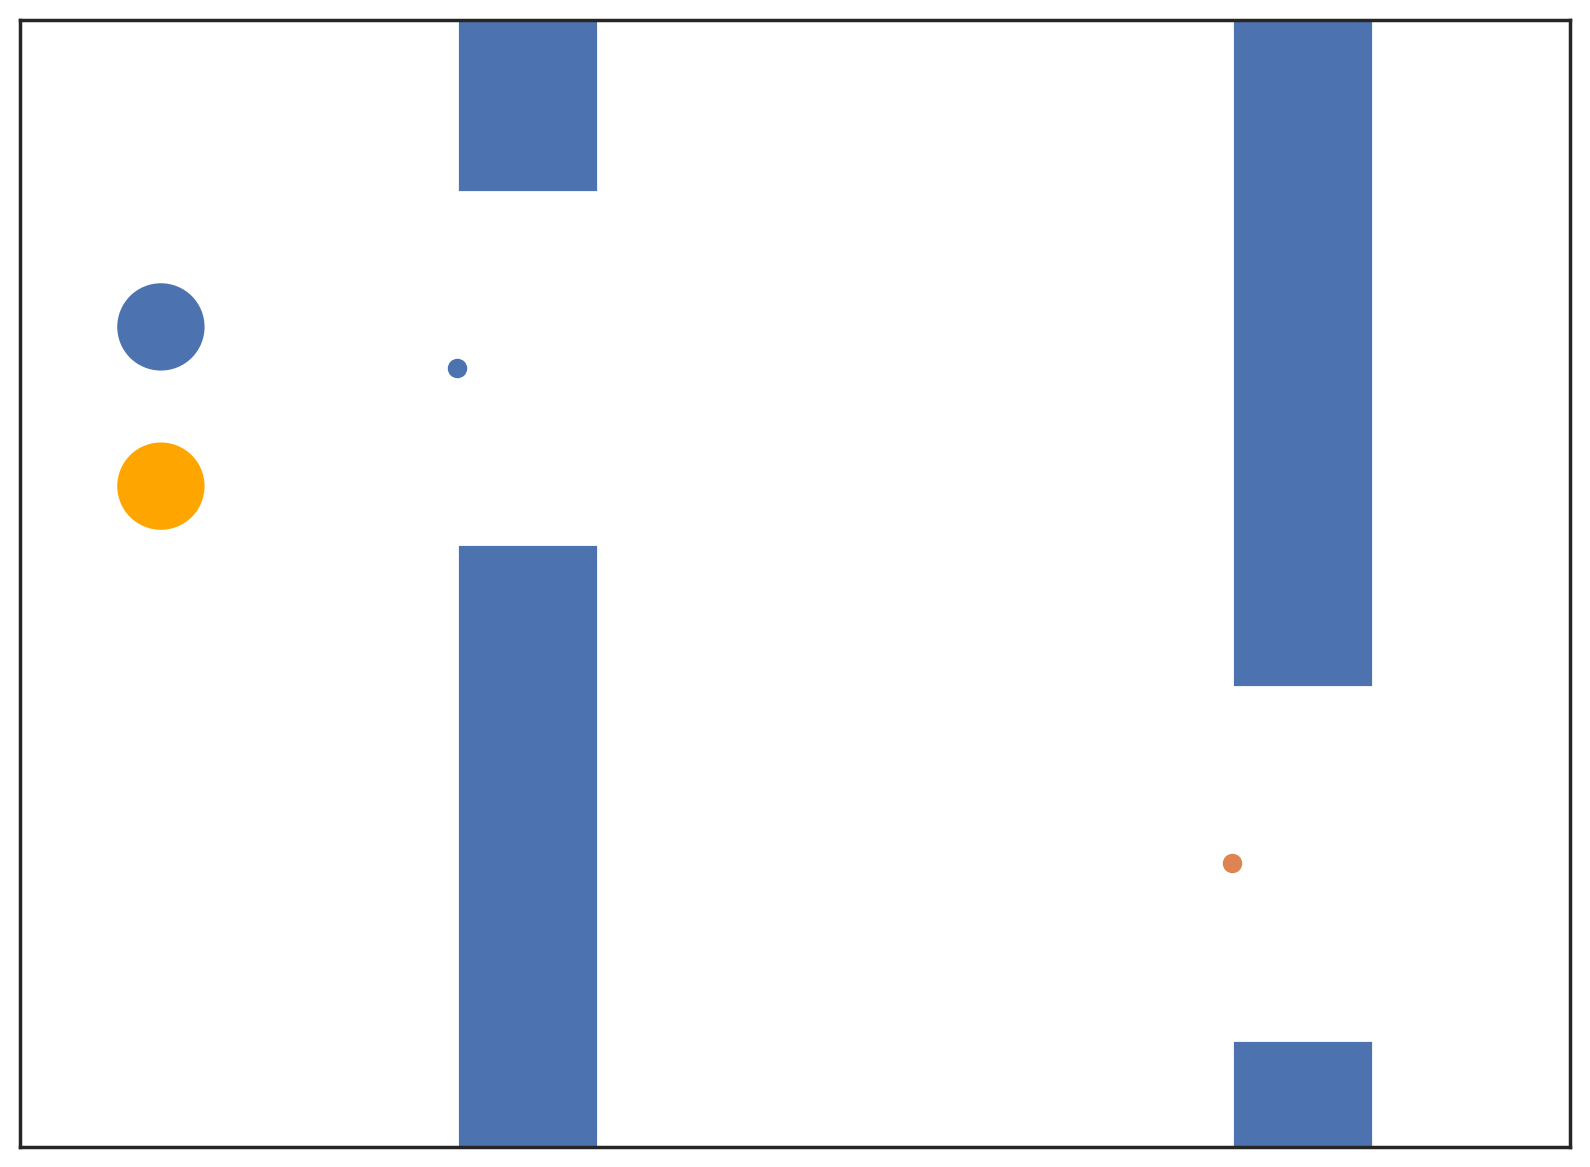
\includegraphics[width=\linewidth]{00023.png}
        \caption{Cuadro 0: Posición inicial.}
    \end{subfigure}%
    ~\hfill
    \begin{subfigure}[t]{0.25\linewidth}
        \centering
        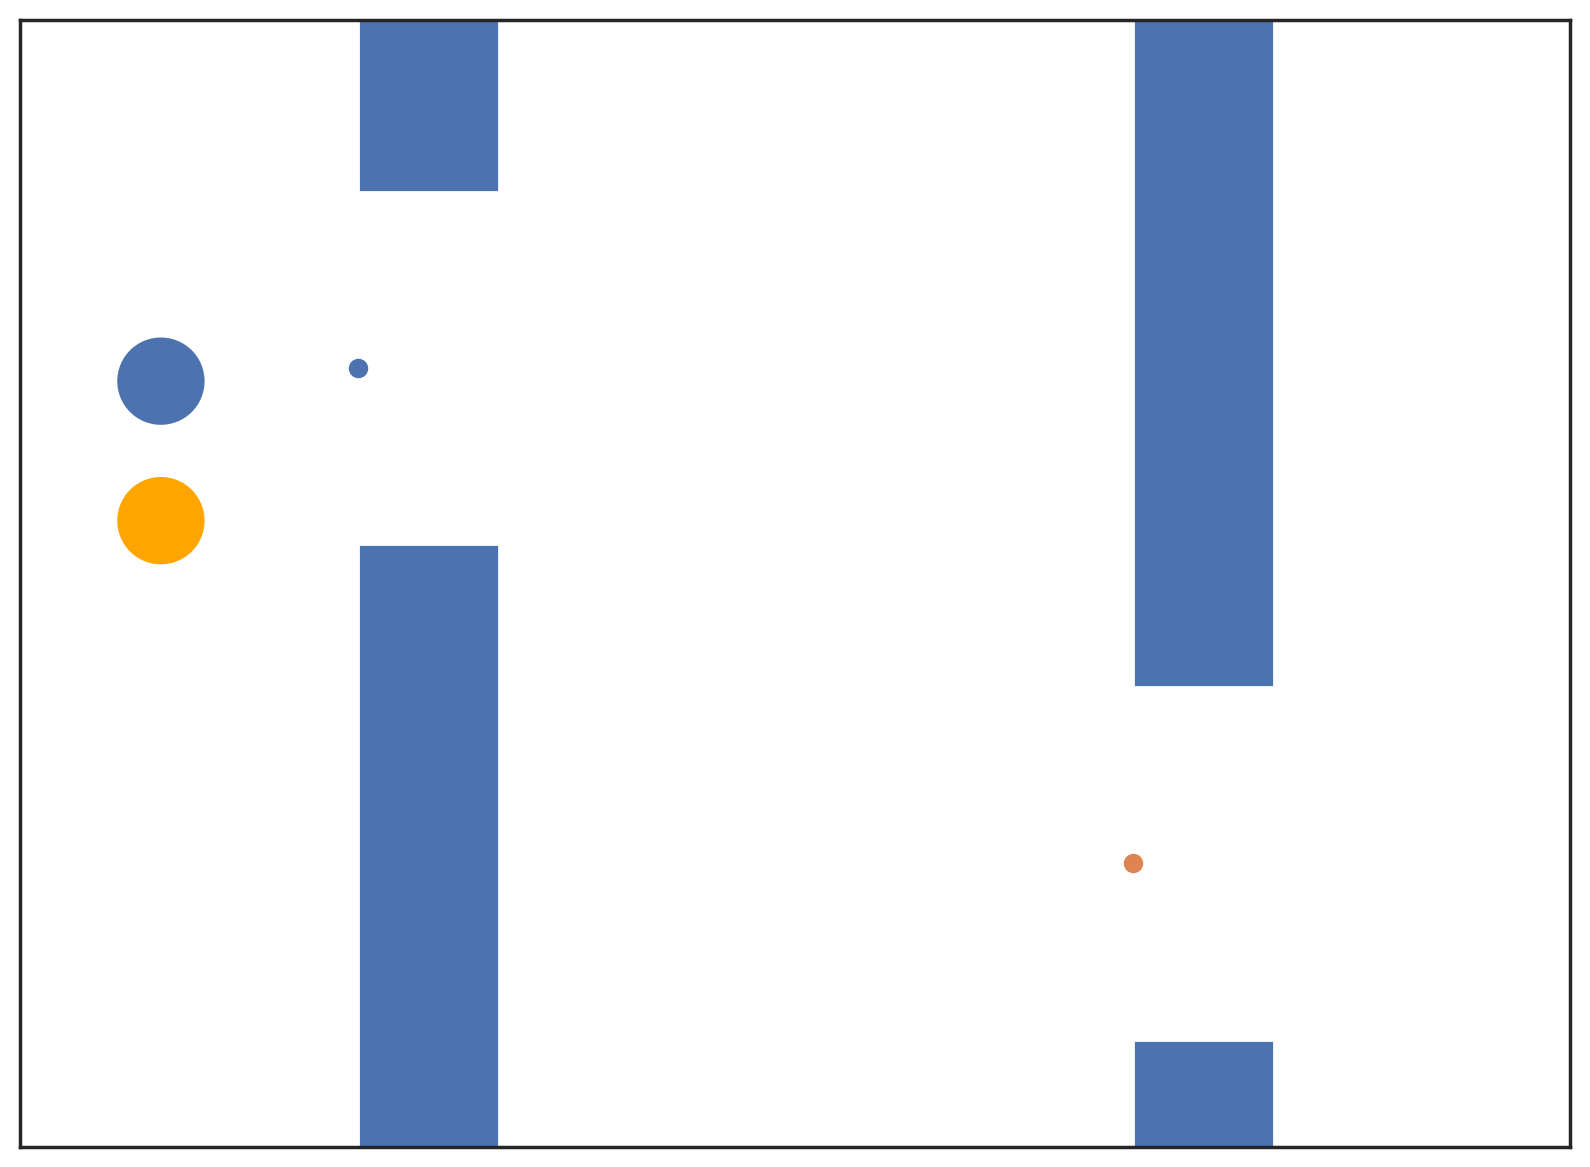
\includegraphics[width=\linewidth]{00030.png}
        \caption{Cuadro 7: La neurona de naranja se activa y hace que aleteé.}
    \end{subfigure}%
    ~\hfill
    \begin{subfigure}[t]{0.25\linewidth}
        \centering
        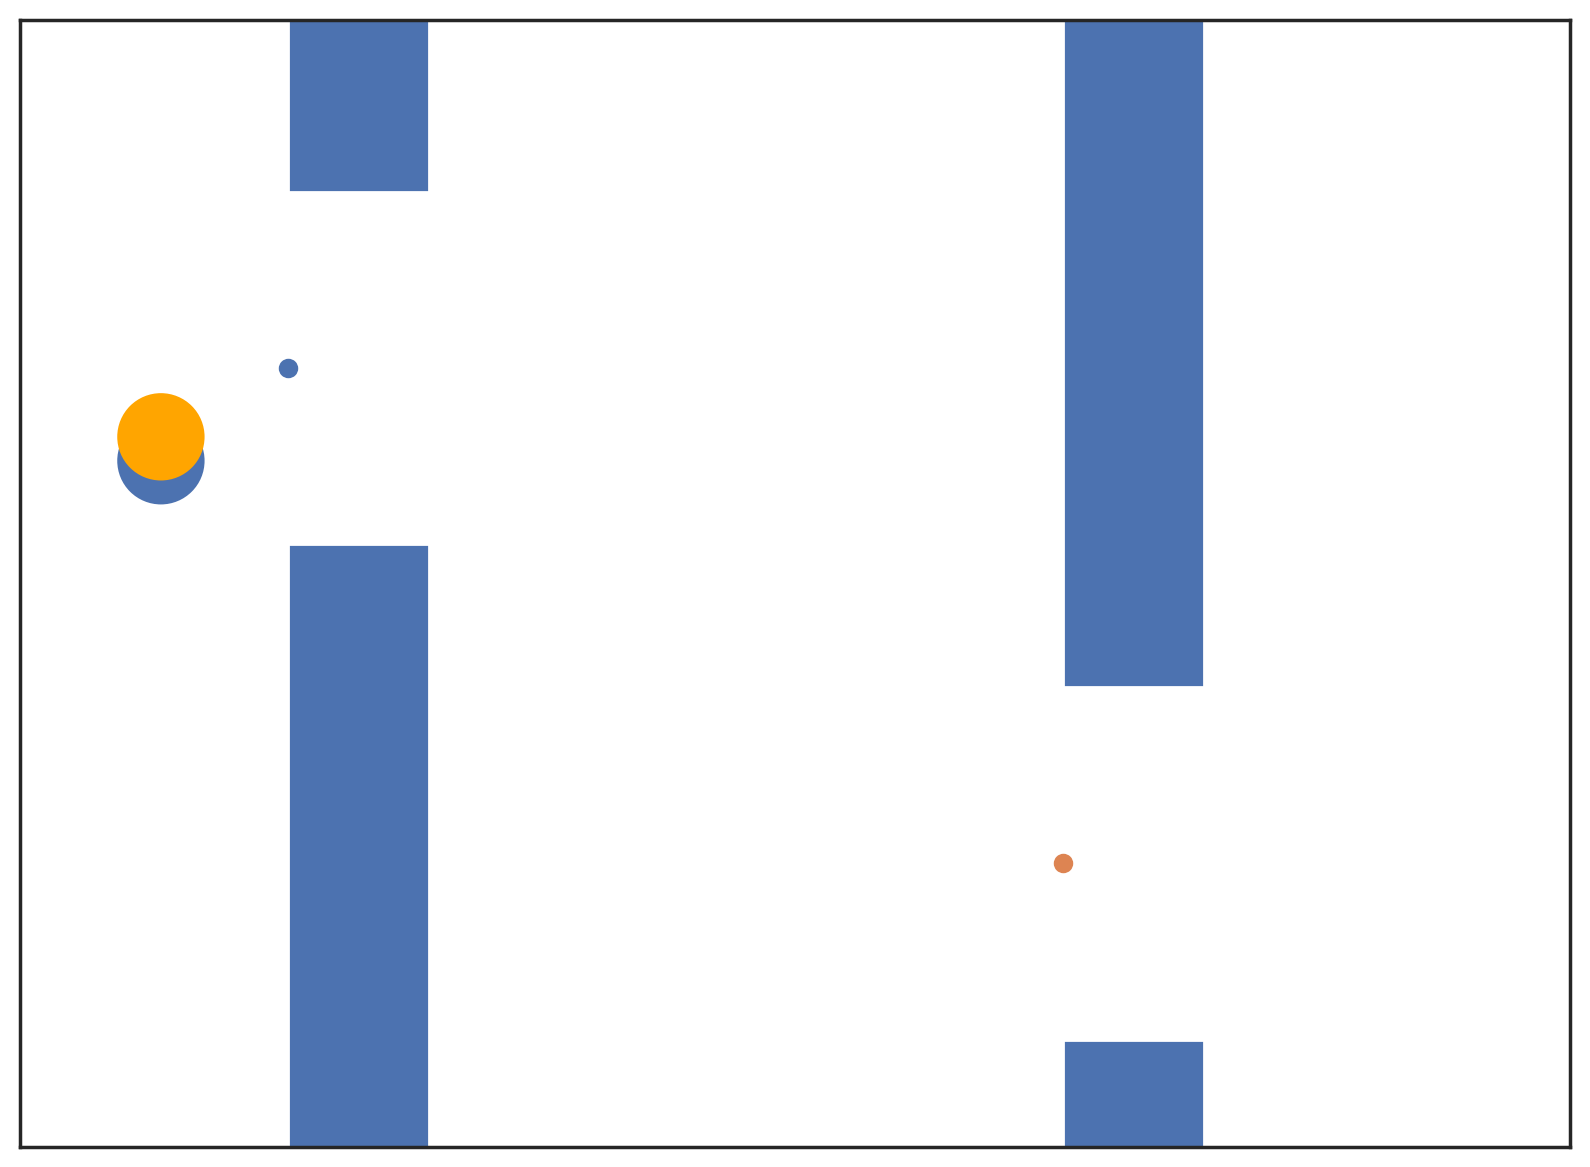
\includegraphics[width=\linewidth]{00035.png}
        \caption{Cuadro 12: La neurona de azul se activa.}
    \end{subfigure}%
    ~\hfill
    \begin{subfigure}[t]{0.25\linewidth}
        \centering
        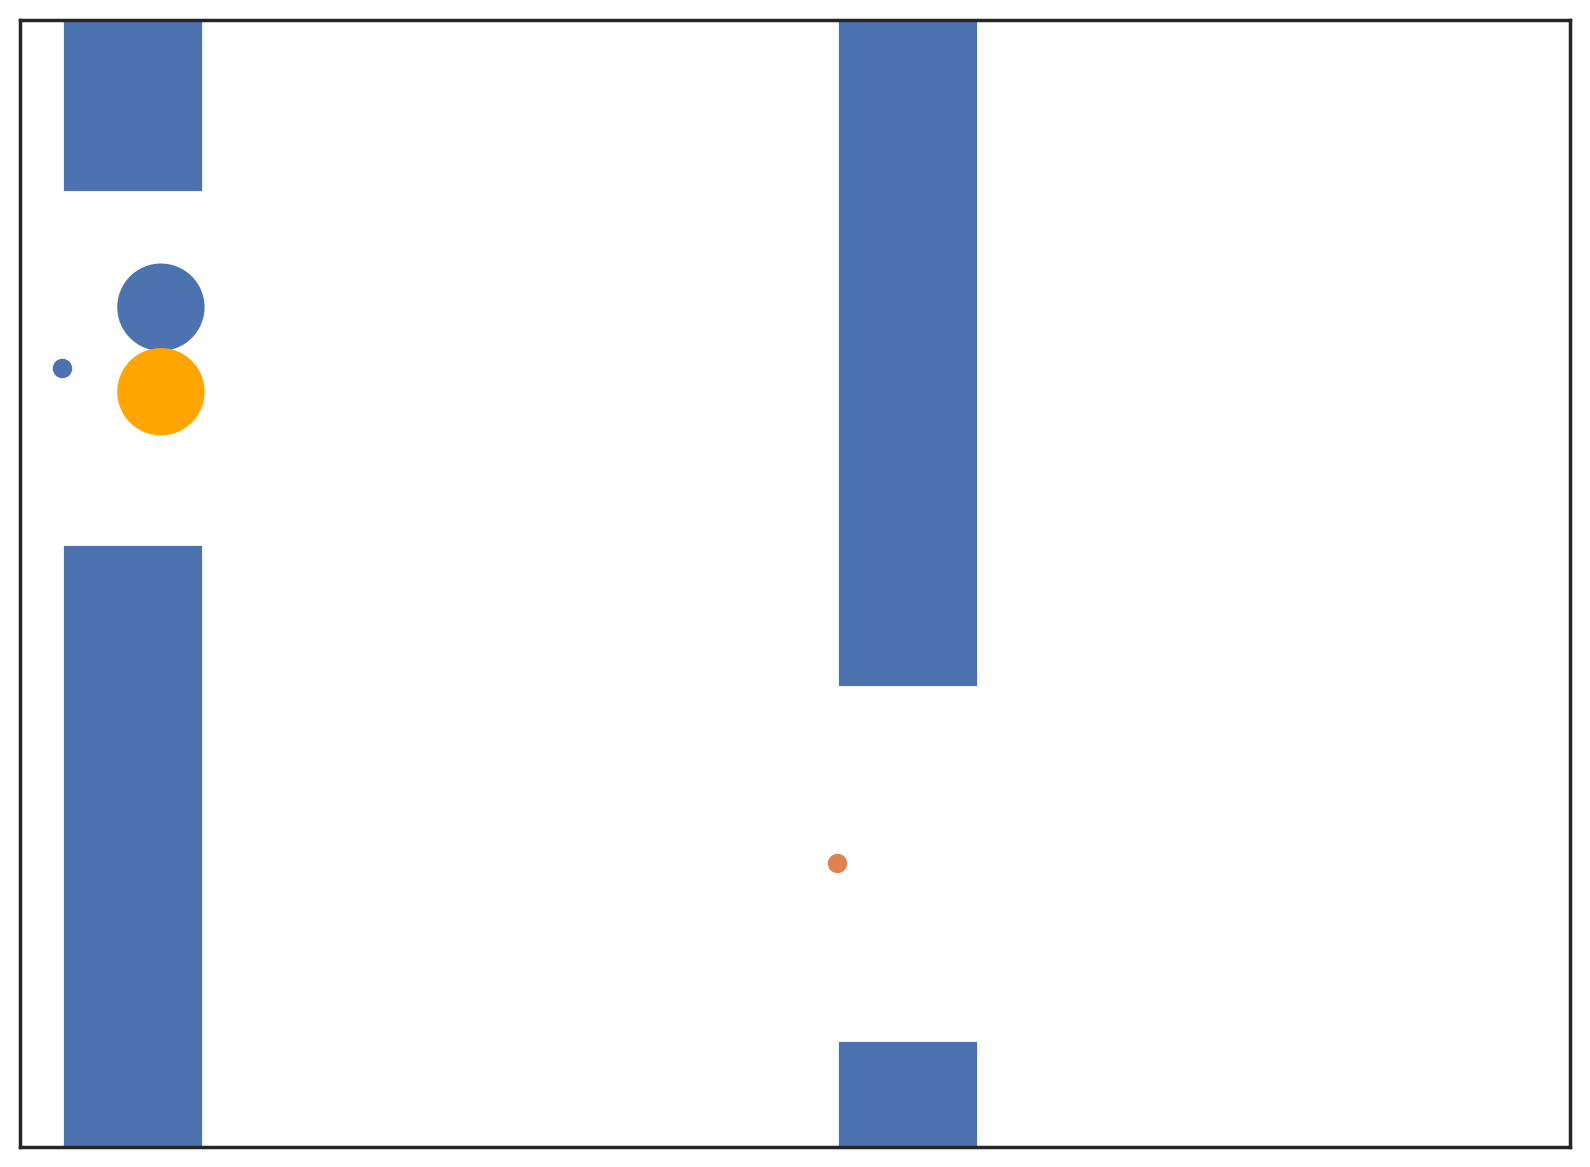
\includegraphics[width=\linewidth]{00051.png}
        \caption{Cuadro 28: Ambos pasan el obstáculo}
    \end{subfigure}%
    \caption{Cuadros selectos de una población experta de dos pájaros, representados por círculos de colores. Los puntos en las aperturas de las tuberías (rectángulos) representan la ubicación que usan los pájaros para calcular su distancia.}
    \label{fig:evol}
\end{figure*}

El encontrar un balance adecuado entre individuos fuertes y débiles es vital para que nuestras poblaciones evolucionen de la manera deseada: si el torneo es muy pequeño, se colarán muchos individuos débiles. Por otro lado, si es muy grande los individuos fuertes siempre dominarán, y no habrá suficiente variabilidad genética.

Por lo tanto, realizamos simulaciones para distinto número de participantes, y calculamos el \textit{fitness} promedio para cada generación. Los resultados pueden verse en la \cref{fig:eval_participantes}.

Como era de esperarse, el \textit{fitness} para el torneo con tan sólo 2 participantes es muy bajo, ya que prácticamente no hay presión de selección. Por otro lado, si bien los torneos de 10 y 50 individuos presentan resultados aproximadamente equivalentes, el último sufre de más decrementos bruscos en el \textit{fitness} promedio en comparación al primero. Esto es ocasionado por una falta de diversidad en la población, lo cual es causado a su vez por una presión de selección demasiado grande. Por lo tanto, nos quedamos con un parámetro de 10 participantes por torneo.

\subsection{Población de ejemplo}
Con los parámetros obtenidos anteriormente, entrenamos de manera eficiente a una población de pájaros. Posteriormente, creamos un nuevo mundo con los dos mejores candidatos, y observamos su evolución conforme pasa el tiempo. Renderizaciones de algunas interacciones importantes pueden verse en la \cref{fig:evol}.

Como punto final, notamos que esta población se mantuvo viva por más de 20 minutos, y solo dejaron de jugar porque suspendimos manualmente la ejecución. 

\section{Conclusión}

En este trabajo se hace un breve repaso de los algoritmos bio-inspirados y evolutivos, de los cuales de tres se discute su funcionamiento y algunos de sus casos de uso. Entre estos tres se hace un breve comparativo para justificar la elección del algoritmo de neuroevolución para la elaboración de este proyecto. Para introducir más al lector en el algoritmo de neuroevolución se explican los conceptos básicos de las redes neuronales y como estos se desarrollan con los algoritmos evolutivos.

Nuestro proyecto comprueba que mediante la implementación de un algoritmo de neuroevolución de forma paralela podemos disminuir el tiempo de ejecución del mismo programa de forma secuencial.

De acuerdo a nuestras gráficas (Figura 13) podemos ver que que en la búsqueda de una aptitud de $25$ o superior podemos hacerlo en menos tiempo de forma paralela (con $4$ procesos) que de forma secuencial (usando $1$ proceso). 

Por otro lado, mostramos que es posible entrenar redes neuronales con un método distinto al convencional (gradiente de descenso) utilizando el algoritmo de neuroevolución. Esto se puede comprobar mediante las gráficas de la Figura $12$ y $13$ puesto que el fitness (función de aptitud) es cada vez mayor, asimismo se puede ver de forma experimental visualizando una generación avanzada, puesto que un pájaro puede jugar correctamente como se muestra en la figura $16$. 

\newpage

\onecolumngrid

\bibliographystyle{ieeetr}
\bibliography{bib} 
\end{document}